\chapter{Оптические и радиолокационные исследования нефтяных сликов} \label{chap:2}


Хорошо известно, что поверхностные пленки, подавляя короткие ветровые волны, проявляются на морской поверхности в виде сликов, которые при малых и умеренных ветрах легко регистрируются как оптическими приборами, так и радиолокаторами. Тем не менее, определение характеристик поверхностных загрязнений моря методами дистанционного зондирования остаётся проблемой, далекой от полного решения.

Существуют многочисленные публикации по идентификации естественных и искусственных поверхностных загрязнений на изображениях, полученных радиолокаторами с синтезированной апертурой (РСА), и установлению их связи с теми или иными источниками загрязнений (см., например, \citep{Gade1998, Espedal1996, Espedal1998, Espedal2000}). ``Простота'' идентификации загрязнений привела к созданию оперативных автоматизированных спутниковых систем РСА контроля нефтяных загрязнений на ряде морских акваторий (см., например, \url{http://www.boost-technology.com}). Однако, на РСА изображениях пленки естественного и искусственного происхождения выглядят одинаково, - в виде темных пятен. Кроме этого существует ряд других естественных явлений (локальные штилевые области, области холодной поверхностной воды, проявления градиентов течений), приводящие к локальным депрессиям обратного рассеяния радиоволн, которые могут восприниматься как поверхностные загрязнения \citep{Espedal2000, Kudryavtsev2003}. Существующие методы выделения нефтяных загрязнений на фоне естественных контрастов РСА изображений базируются в основном на текстурном анализе ``пятен'', однако достоверность такой идентификации остается весьма невысокой.

Альтернативным подходом является создание алгоритмов определения параметров загрязнений основанных на оценке величин контрастов слика на одной или нескольких радиолокационных (РЛ) частотах \citep{Ermakov1987} и различном наборе поляризаций излучения/приема РЛ сигнала. Реализация такого подхода, несомненно, требует либо надежных эмпирических соотношений, связывающих РЛ контрасты слика с параметрами поверхностных веществ и скорости ветра, либо модели формирования РЛ контрастов, тестированной на экспериментальных данных. Однако, число систематических натурных экспериментов по исследованию спектральных или РЛ контрастов в сликах, связанных с пленками с известными физико-химическими характеристиками, которые сопровождались бы измерениями параметров окружающей среды, все еще ограничено (см, например, \citep{Ermakov1986, Ermakov1992, Gade1998, Gade1998b}). Более того, измерения контрастов, проведенные одними и теми же методами с одинаковыми веществами и при эквивалентных ветровых условиях, демонстрируют значительный разброс данных.

Кроме этого, в настоящее время существует определенный ``дефицит'' теоретических подходов к моделированию контрастов шероховатости морской поверхности в сликах. Cтрогая теория разработана лишь для коэффициентов гашения волн бесконечно тонкими поверхностными пленками \citep{Levich1959} и пленками конечной толщины \citep{Jenkins1997}. Эти коэффициенты определяют скорость диссипации энергии, которая является одним из элементов уравнения баланса энергии ветровых волн. Существующие модели контрастов спектра ветрового волнения (см., \citep{Ermakov1987, Ermakov1992, Alpers1989, Gade1998}) в качестве диссипация энергии в пленках используют модель \citep{Levich1959}, а отличие этих моделей друг от друга состоит в предположениях о важности тех или иных источников энергии в уравнении баланса энергии волн и их параметризации.

Помимо РЛ изображений, ещё более полувека назад Кокс и Манк~\citep{Cox1954, Cox1954a}, использовали самолётные фотографии солнечного блика для изучения влияния искусственных плёнок на значения СКН. Позже, возможность наблюдения поверхностных сликов по оптическим изображениям солнечного блика из космоса была продемонстрирована в многочисленных работах, например \citep{Brekke2005, Chust2007, Hu2009}.

В этой главе показываются возможности нового разработанного метода, описанного в Главе~\ref{chap:1}, для численного восстановления аномалий СКН по яркости морской поверхности, покрытой нефтяными плёнками, в солнечном блике. Также приводится совместный анализ полученных результатов с данными радиолокаторов с синтезированием апертуры (РСА), и раскрываются преимущества синергетического подхода в исследовании поверхностных сликов.



\section{Нефтяные плёнки природного происхождения} \label{sec:2.1}


Для начала обратимся к изображениям MODIS Мексиканского залива. На одном из приведённых ниже изображений яркости солнечного блика (Рисунок~\ref{fig:2.1}) различимы следы разлива нефтепродуктов природного происхождения. Изучая эти изображения, Ху с соавторами \citep{Hu2009}, обнаружили, что контрасты поверхностных сликов в солнечном блике бывают как яркими, так и тёмными. Контрасты сликов, как говорится в статье \citep{Hu2009}, зависят от угла между направлением визирования и направлением зеркального отражения $\theta _{m} $. В рассматриваемом случае контрасты сликов меняли знак при $\theta _{m} \approx 12^{0} $, оставаясь положительными при меньших углах и отрицательными -- при больших. Хотя Ху и соавторы в своей статье \citep{Hu2009} описали наблюдаемое явление, но не смогли обобщить его и рекомендовали провести дальнейшие исследования. Обобщение этого явления и описание причин его возникновения было проделано в данной работе.

Фрагмент исходного изображения MODIS (MODIS/Terra, 2 Июня 2005, 16:55 GMT), анализированного в \citep{Hu2009} приведён на Рисунке~\ref{fig:2.1} (верхний левый). На данном изображении видно большое количество ``закрученных'' структур. Эти структуры и есть слики, образованные из природно-сформировавшейся нефти, выделяющейся естественным образом из так называемых грифонов на морском дне. Контрасты яркости $\tilde{B}/B_{0} $, представленные на Рисунке~\ref{fig:2.1} (верхний правый), имеют различные знаки по разным сторонам 92-го градуса западной долготы. Происхождение этой зоны, так называемой зоны инверсии контрастов, следует из определения передаточной функции \eqref{eq:1.7}. Как уже утверждалось ранее, возникновение воображаемой линии, делящей область солнечного блика на две части, где вариации СКН приводят к отрицательным и положительным контрастам, следует из решения уравнения: $T(x,y)=0$ (см. также Рисунок~\ref{fig:5}, где представлены модельные расчёты).



\begin{figure}[!thb]
 \includegraphics[width=\linewidth]{fig2_1}
 \floattitle{(верхний левый) Фрагмент изображения с прибора MODIS/Terra (Июнь, 2, 2005, 16:55 GMT) на длине волны 645\textit{нм} (красный канал) Мексиканского залива с особенностями проявления нефтяных сликов в солнечном блике. (верхний правый) Контрасты яркости $\tilde{B}/B$. (нижний левый) Передаточная функция. (нижний правый) Восстановленные контрасты СКН}
 \caption{Фрагмент изображения, полученного с прибора MODIS/Terra (Июнь, 2, 2005, 16:55 GMT)}
 \label{fig:2.1}
\end{figure}


Рисунок~\ref{fig:2.1} (нижний левый) показывает передаточную функцию, рассчитанную по уравнениям \eqref{eq:1.7}, \eqref{eq:1.8} и \eqref{eq:1.9} для сглаженного поля яркости солнечного блика. Контрасты $\tilde{s}^{2} /s_{0}^{2} $, полученные по полю яркости, изображены на Рисунке~\ref{fig:2.1} (нижний правый). В окрестности зоны инверсии контрастов, где передаточная функция стремится к нулю: $T\to 0$, она проявляется как область сингулярных, очень больших значений, и, как следствие, не имеет физического значения.

После применения алгоритма, контрасты, ассоциируемые с нефтяными сликами, теперь систематически отрицательны. Также можно отметить другие особенности в контрастах СКН (как отрицательные, так и положительные), вызванные вариациями в поле ветра на внутренних масштабах блика. Контрасты СКН нефтяных сликов составляют $\tilde{s}^{2} /s_{0}^{2} \approx 0.3-0.4$, что эквивалентно уменьшению СКН внутри слика в 1.5 раза. Эта оценка ниже оценки, приведённой Коксом и Манком \citep{Cox1954a} (2-2.5 раза), для поверхностных сликов, образованных смесью рыбьего жира, моторного масла и дизельного топлива. Также стоит обратить внимание, что упругость такой поверхностной плёнки меньше упругости смеси рыбьего жира, которая составляет около 30\textit{мН/м} и, предположительно больше упругости нефтепродуктов, которая плохо изучена (одно из предложенных значений \textit{E}=4\textit{мН/м}, из личного общения с С.~Ермаковым). Поскольку упругость поверхностных плёнок определяет подавление коротких ветровых волн, меньшее значение упругости должно приводить к меньшим контрастам в сликах (см. раздел \ref{sec:2.3} и Рисунок~\ref{fig:2.10} ниже).

На Рисунке~\ref{fig:2.2} (слева) показан увеличенный фрагмент Рисунка~\ref{fig:2.1} (нижний левый), содержащий ``индивидуальные'' нефтяные слики, а на Рисунке~\ref{fig:2.2} (справа) представлена зависимость контрастов СКН от скорости ветра по 12-и выбранным нефтяным сликам. Оценки скорости ветра были проведены по значениям $s_{0}^{2} $, используя эмпирические соотношения Кокса и Манка \citep{Cox1954, Cox1954a}. Также на Рисунке~\ref{fig:2.2} приведены контрасты СКН биогенных сликов, полученные Коксом и Манком \citep{Cox1954a}, которые определены как отношение регрессионных прямых СКН для чистой и сликовой поверхности моря. Как следует из Рисунка~\ref{fig:2.2} (справа), при малых скоростях ветра, наблюдаемые контрасты СКН нефтяных сликов находятся ниже уровня контрастов, обнаруженных Коксом и Манком \citep{Cox1954, Cox1954a} для сликов из смеси рыбьего жира. Отсюда можно заключить, что контрасты нефтяных сликов систематически ниже контрастов рыбьего жира.



\begin{figure}[!thb]
 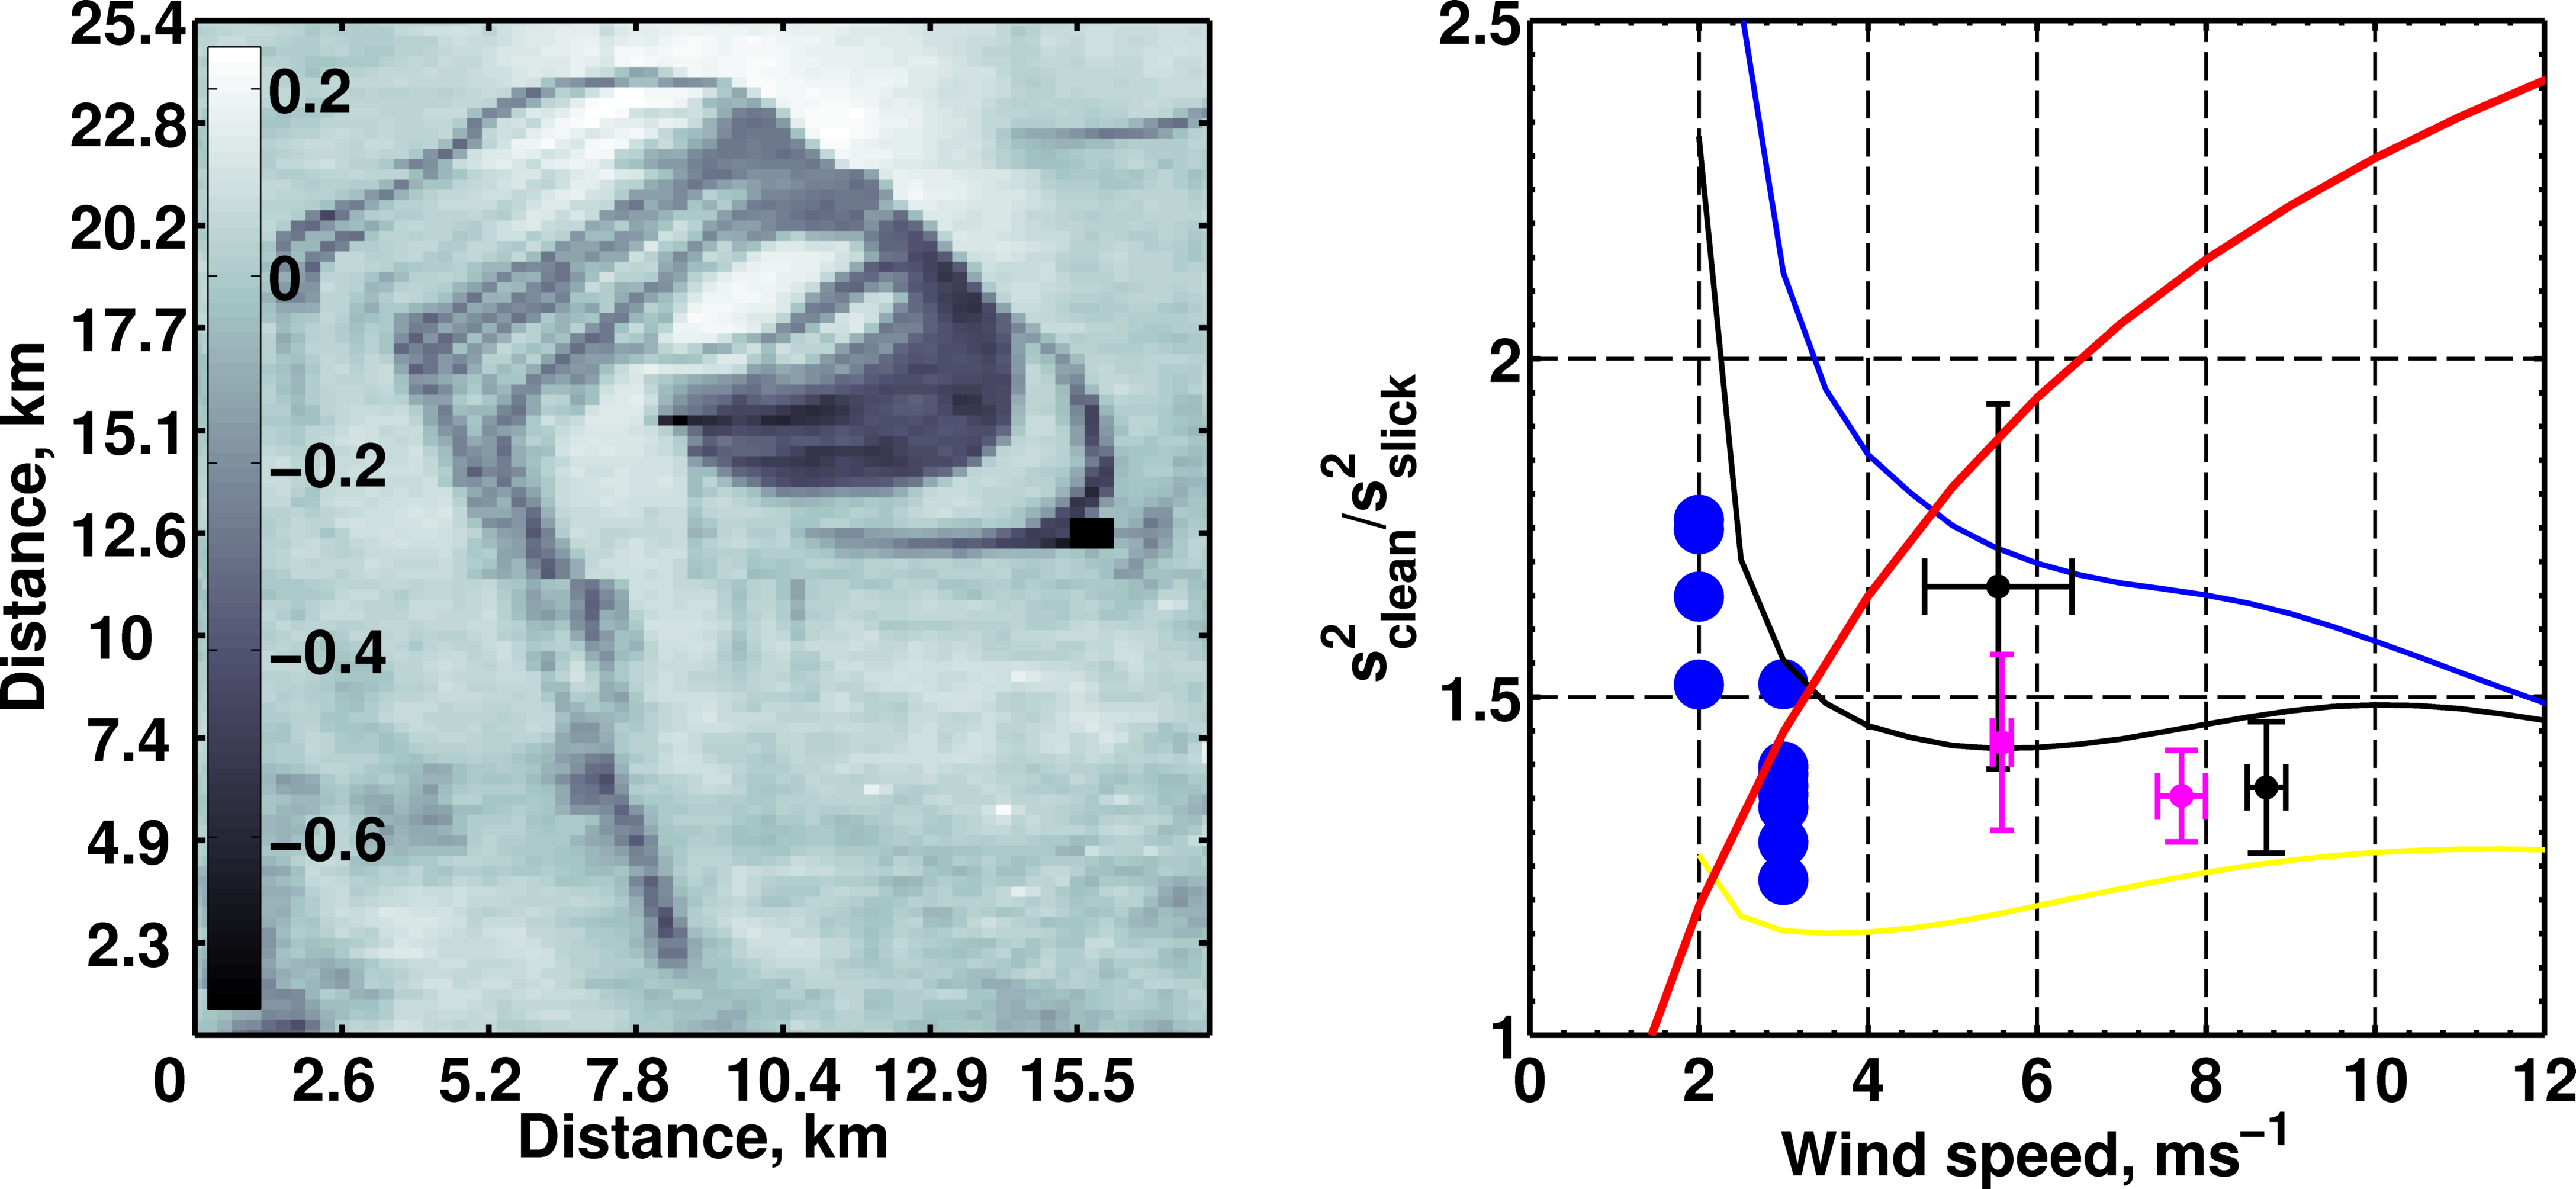
\includegraphics[width=\linewidth]{fig2_2}
 \floattitle{(cлева) Увеличенный фрагмент контрастов СКН, изображённых на Рисунке~\ref{fig:2.1}, содержащем ``индивидуальные'' нефтяные слики. (справа) Контрасты СКН нефтяных сликов, полученных по изображению MODIS на Рисунке~\ref{fig:2.1} (синие точки при скоростях ветра 2-3\textit{м/c}), по изображению MERIS на Рисунках~\ref{fig:2.6} и \ref{fig:2.8} (фиолетовые точки с ошибками), и по изображениям MODIS (чёрные точки с ошибками). Красной кривой показаны контрасты СКН рыбьего жира из результатов Кокса и Манка \citep{Cox1954, Cox1954a}. Желтая, чёрная и синяя кривые отражают результаты моделирования контрастов СКН, вызванных тонкими поверхностными сликами с 5, 15 и 30\textit{мН/м}, соответственно}
 \caption{Увеличенный фрагмент контрастов СКН, изображённых на Рисунке~\ref{fig:2.1}, содержащем ``индивидуальные'' нефтяные слики, и зависимость контрастов от скорости ветра}
 \label{fig:2.2}
\end{figure}


\section{Катастрофические нефтяные загрязнения}


Катастрофический разлив нефти в результате взрыва на нефтяной платформе Дипвотер Хорайзон (англ. Deepwater Horizon) в Мексиканском заливе выбран для дальнейшей иллюстрации работы предложенного метода. На Рисунке~\ref{fig:2.3} приводятся изображения MODIS (MODIS/Terra, Май, 24, 2010, 16:45 GMT) и MERIS (MERIS/Envisat, Май 24, 2010, 16:17 GMT) в красных каналах (645\textit{нм} и 681\textit{нм}, соответственно). Стоит отметить, что одно изображение MODIS/Terra полностью не покрывает нефтяной слик. Поэтому на Рисунке~\ref{fig:2.3b} приводится композит двух изображений MODIS/Terra, полученных 16:45 и 16:50 GMT. Разница во времени между рассматриваемыми снимками MERIS и MODIS около получаса, поэтому стоит полагать, что ``геометрия'' нефтяного загрязнения на поверхности Океана не должна была сильно измениться за этот промежуток. Однако, в результате различных условий наблюдения и положения Солнца, ``геометрия'' слика на изображениях MODIS и MERIS в солнечном блике всё-таки отличается.

Рассматриваемые изображения обработаны по методологии, изложенной в предыдущей главе (см.~Глава~\ref{chap:1}, раздел~\ref{sec:1.3}). Поля средней яркости солнечного блика $B_{0} $ (масштаб осреднения 30x30~км${}^{2}$) для данных MERIS и MODIS представлены на Рисунках~\ref{fig:2.4a} и \ref{fig:2.4b}. Передаточная функция для данных MODIS, показана на Рисунке~\ref{fig:2.4d}, напрямую рассчитывается из осреднённого поля яркости (следуя уравнениям \eqref{eq:1.7}, \eqref{eq:1.8} и \eqref{eq:1.9}). Обратите внимание, что на рисунке проявляется наклонная линейная неоднородность, образованная в результате слияния двух изображений MODIS/Terra. Для оценки передаточной функции данных MERIS использовалось направление ветра по данным NCEP, а затем проводился расчёт СКН, используя уравнение \eqref{eq:1.15}. Передаточная функция для данных MERIS приведена на Рисунке~\ref{fig:2.4c}.



\begin{figure}[H]
	\centering
	\begin{minipage}{.93\textwidth}
		\subcaptionbox{\label{fig:2.3a}}
		{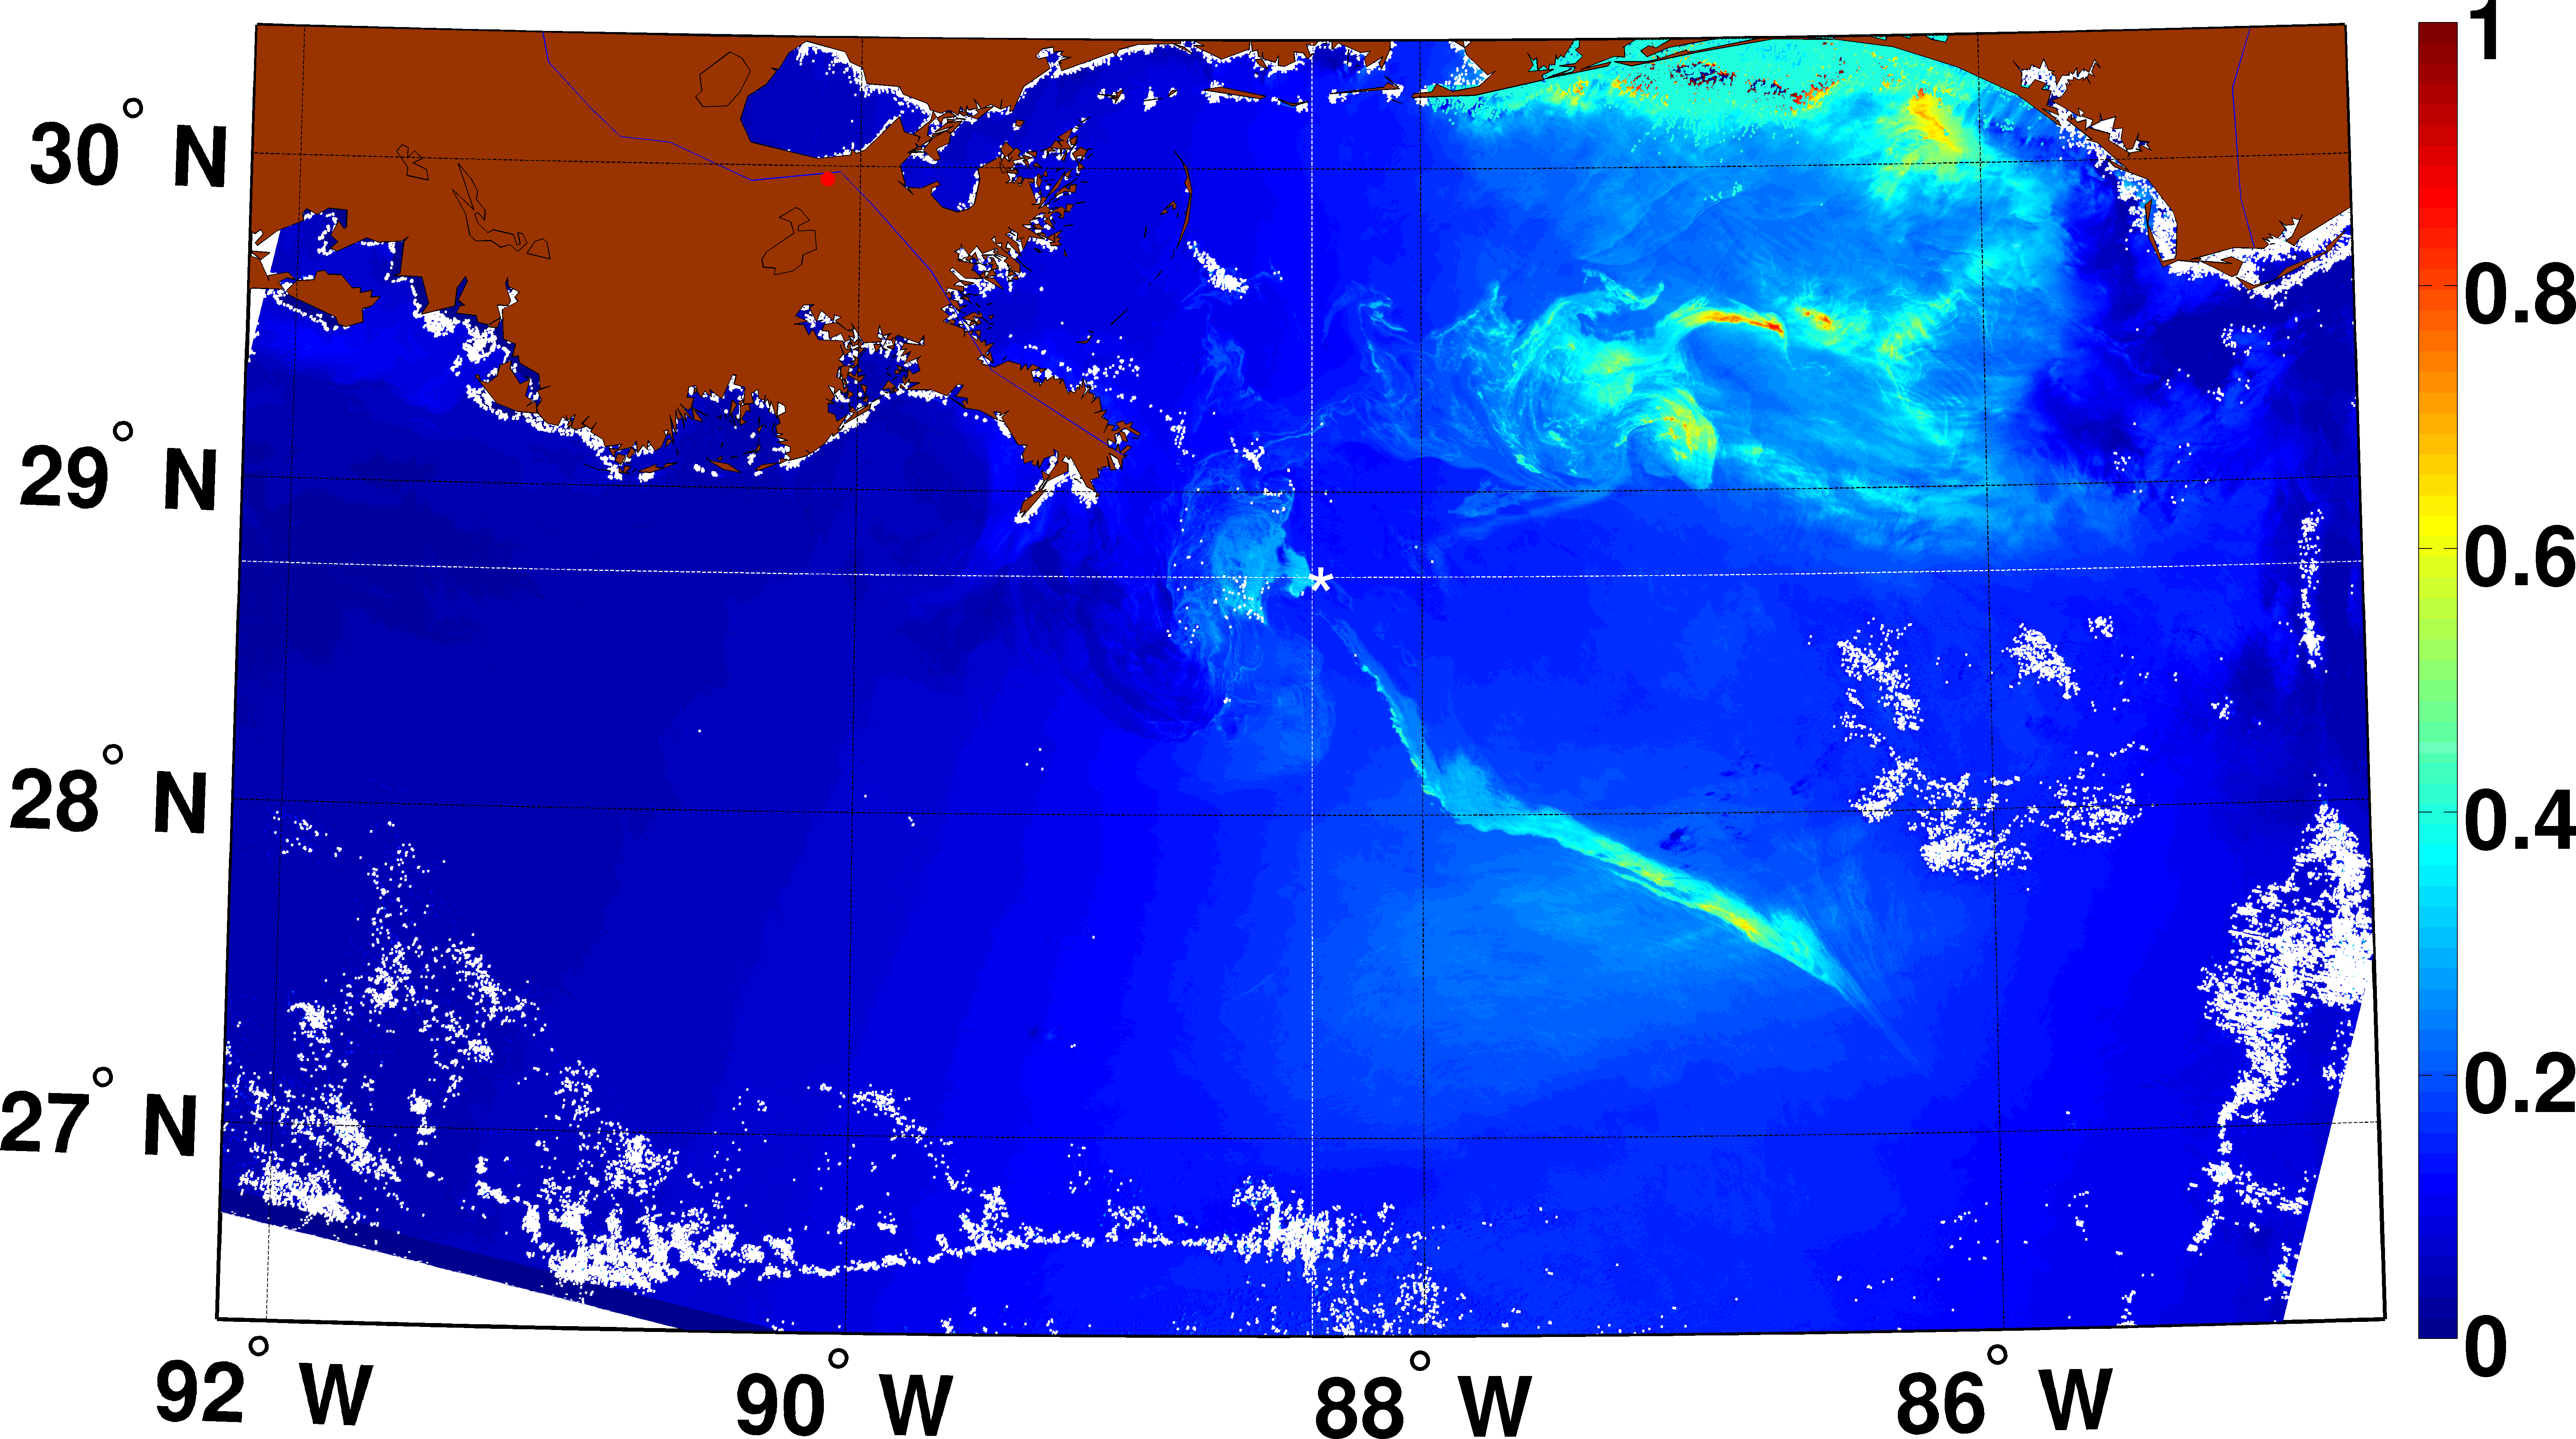
\includegraphics[width=\linewidth]{fig2_3a}}
	\end{minipage}
   	\hfill
	\\
	\begin{minipage}{.95\textwidth}
		\subcaptionbox{\label{fig:2.3b}}
		{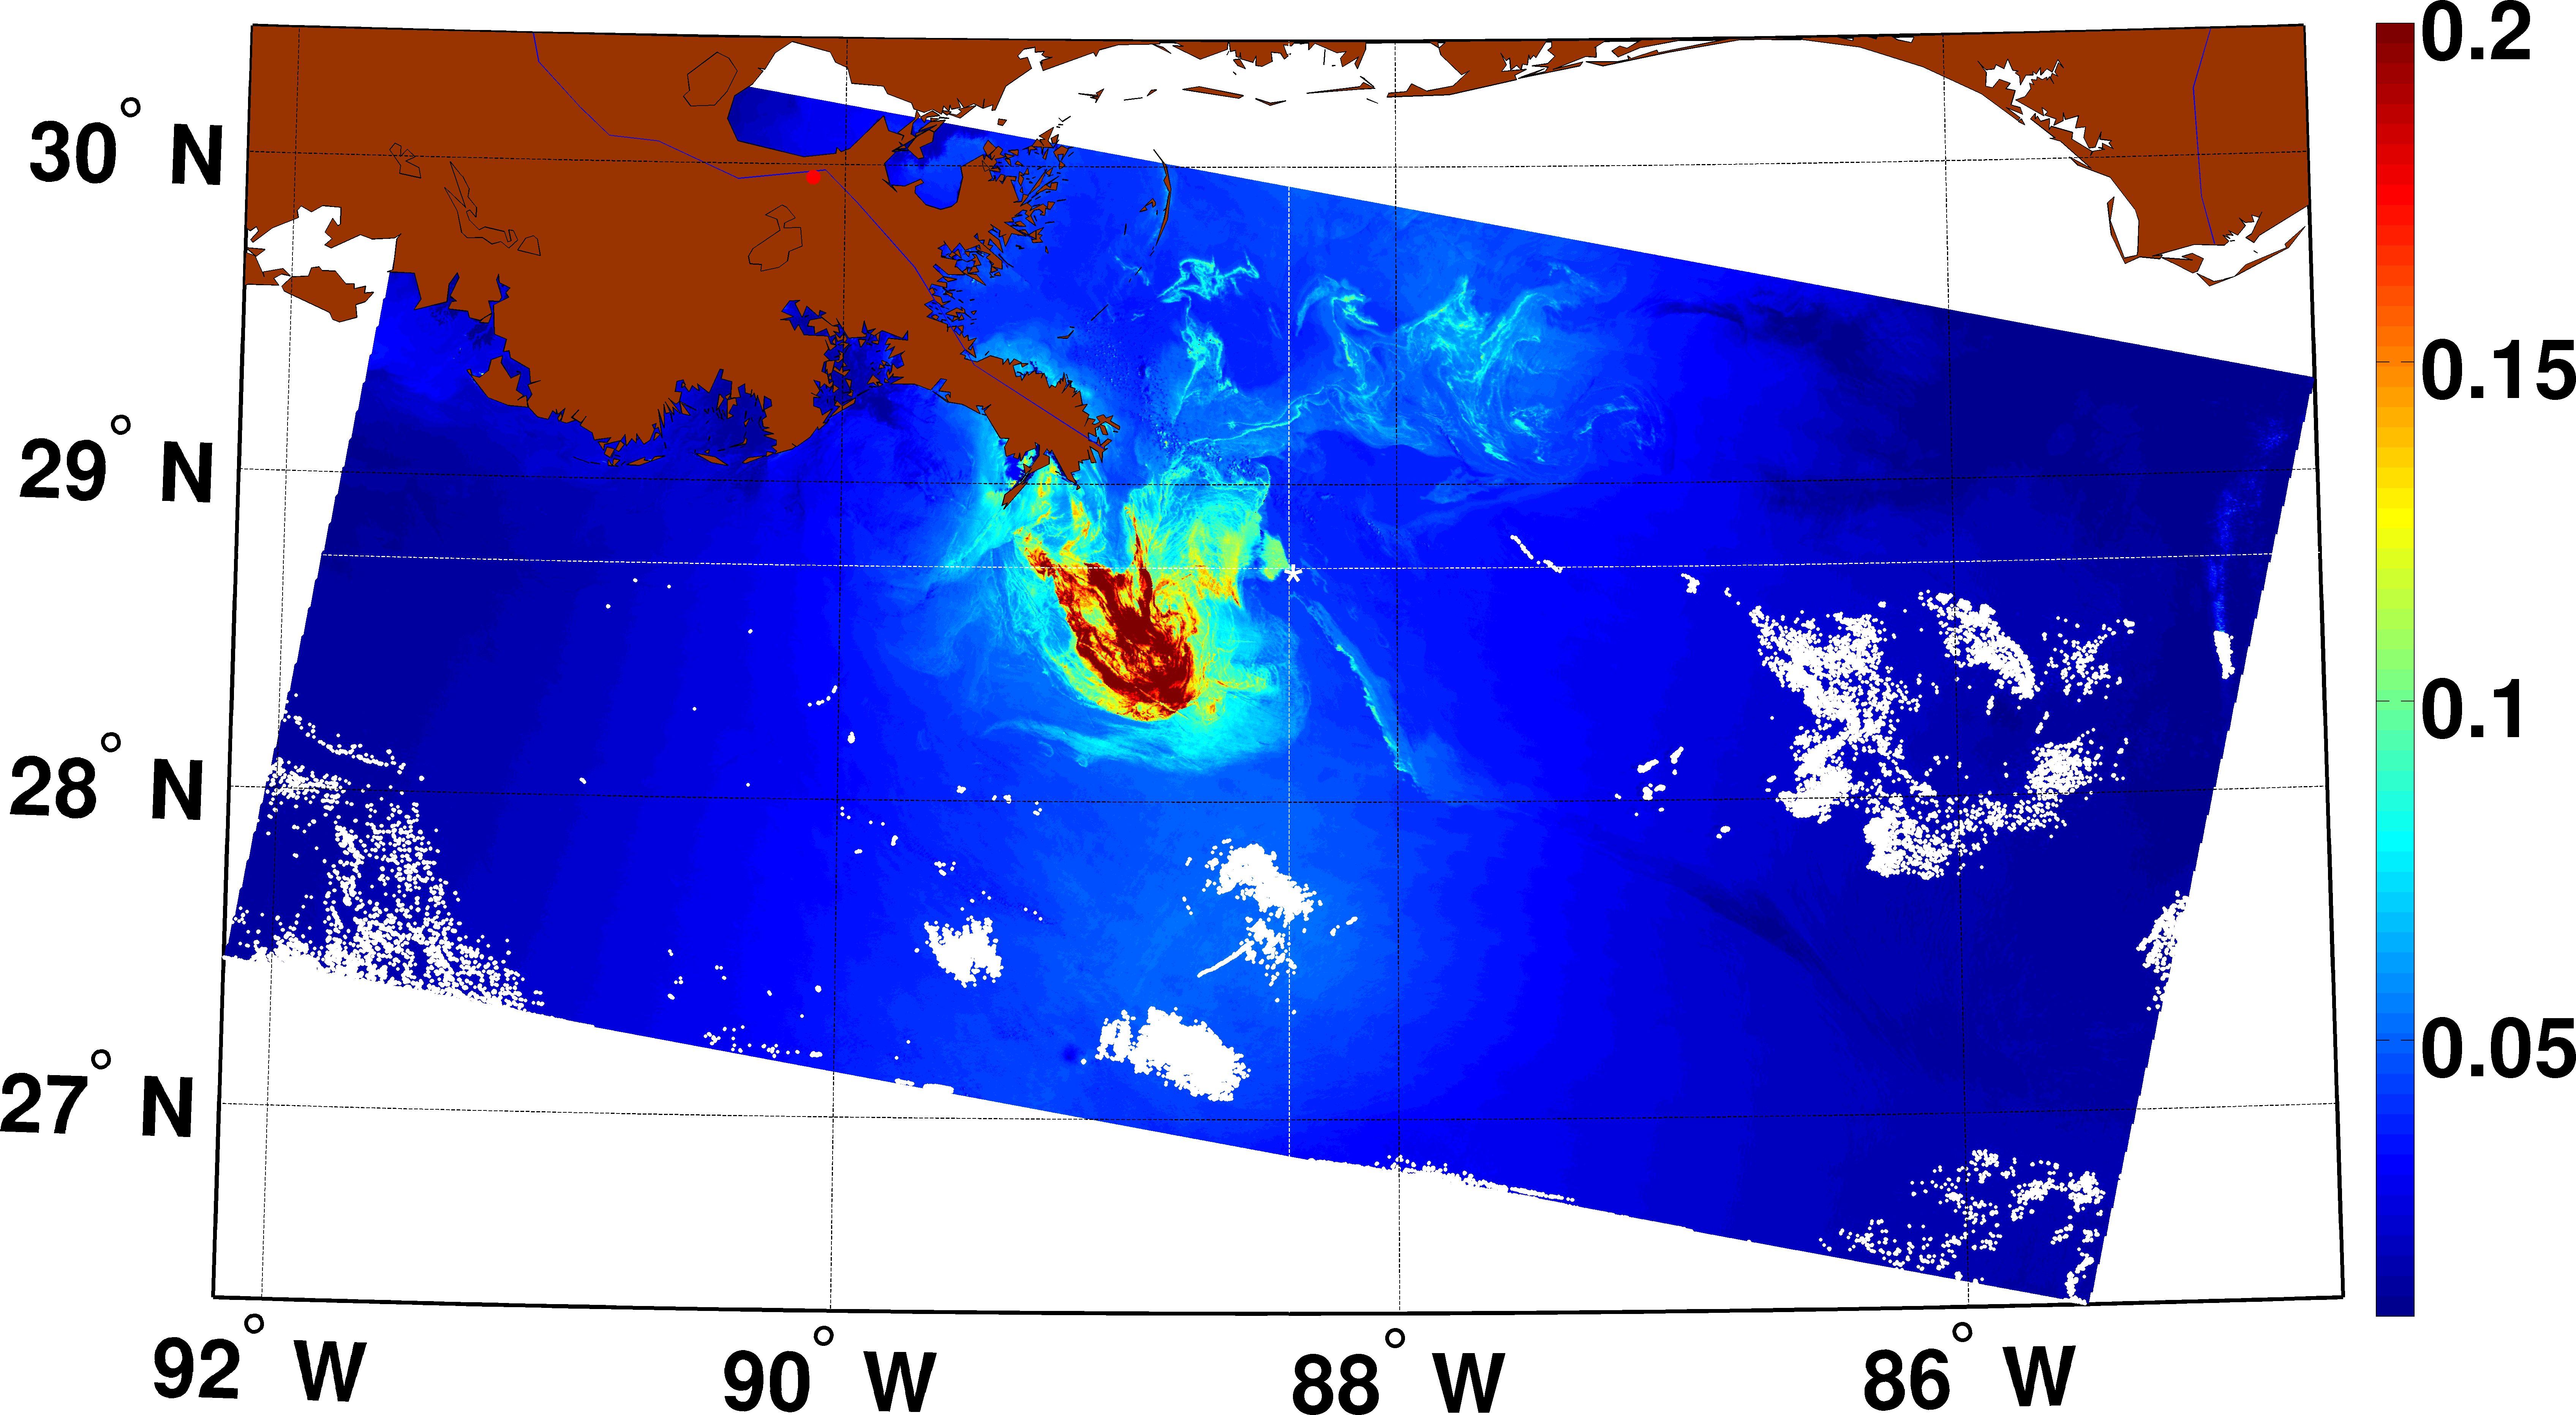
\includegraphics[width=\linewidth]{fig2_3b}}
	\end{minipage}
    \\
    \floattitle{Цветовая шкала приведена в относительных единицах и характеризует яркость изображений. Маска облаков выделена белым цветом, а маска земли коричневым. Координаты нефтяной платформы Deepwater Horizon: 28.73${}^\circ$СШ, 88.38${}^\circ$ЗД}
    \caption{Фрагмент исходного изображения MERIS/Envisat в красном канале (681\textit{нм}), полученное 24 Мая 2010, 16:17 GMT (a) и композитное изображение двух снимков MODIS/Terra в красном канале (645\textit{нм}), полученное 24 Мая 2010, 16:45 и 16:50 GMT (б)}
    \label{fig:2.3}
\end{figure}



\begin{figure}[H]
   	\centering
	\begin{minipage}{.47\textwidth}
	    \subcaptionbox{\label{fig:2.4a}}
		{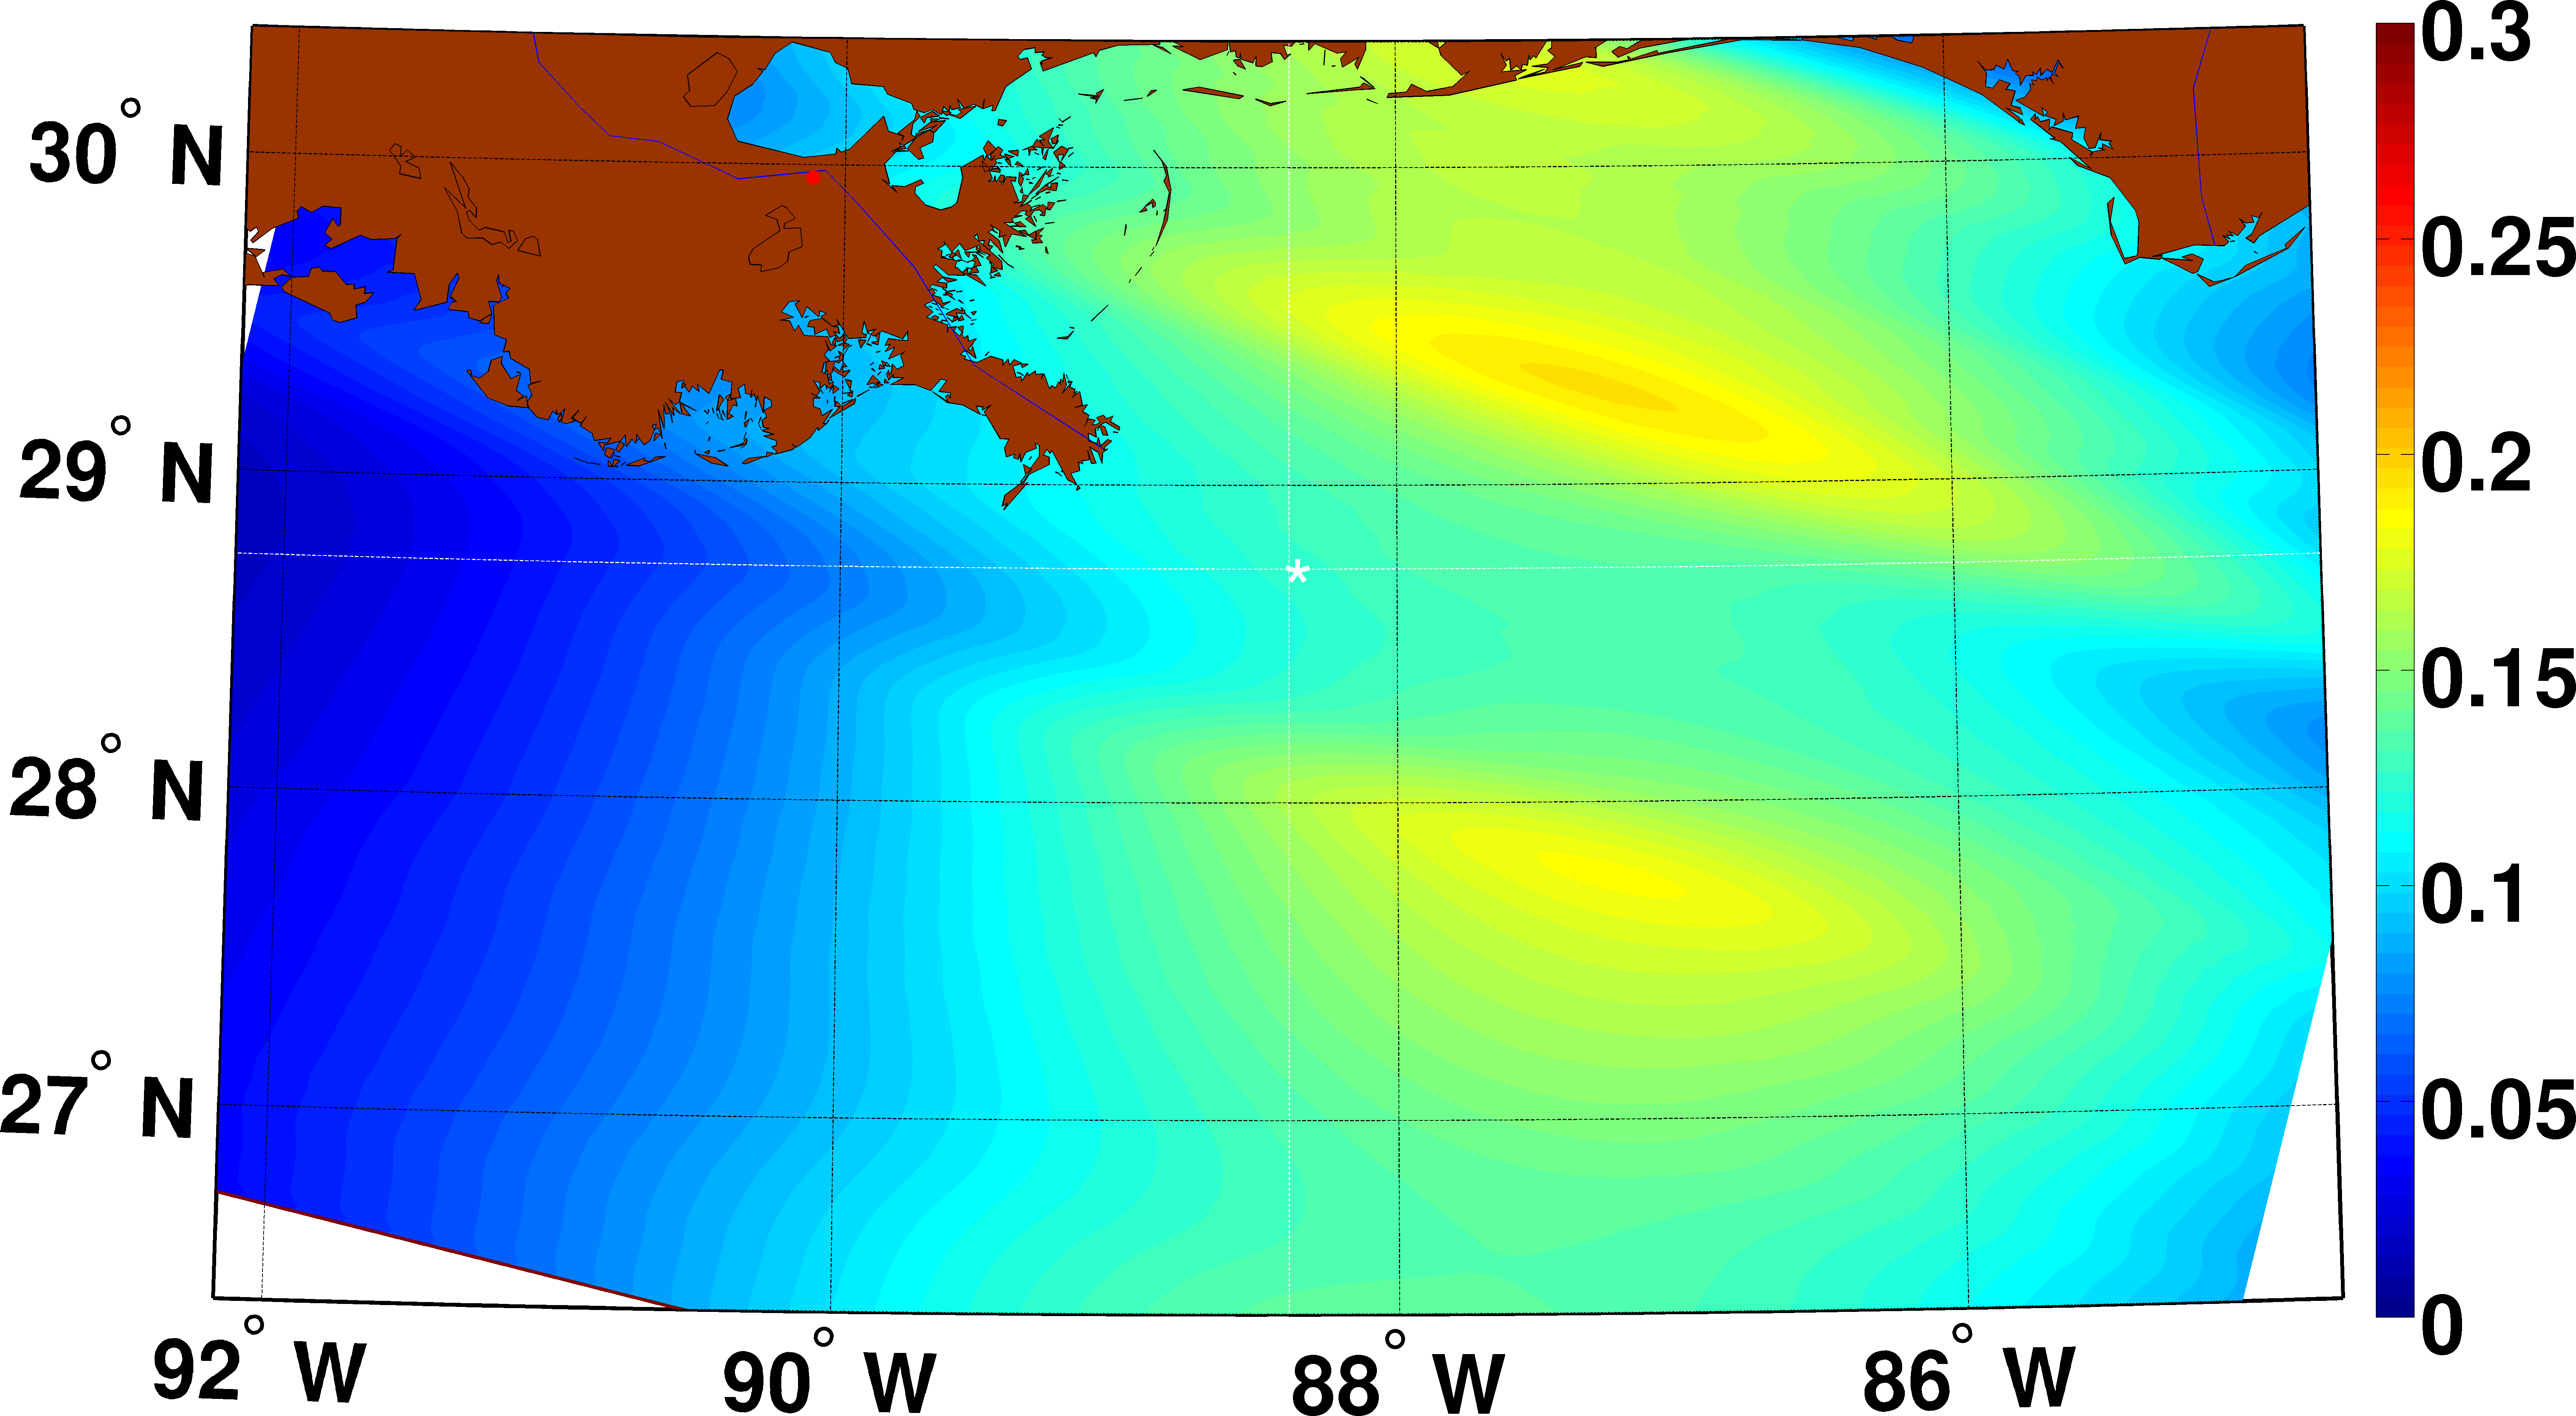
\includegraphics[width=1\linewidth]{fig2_4a}}
	\end{minipage}
	\hfill
	\begin{minipage}{.47\textwidth}
	    \subcaptionbox{\label{fig:2.4b}}
		{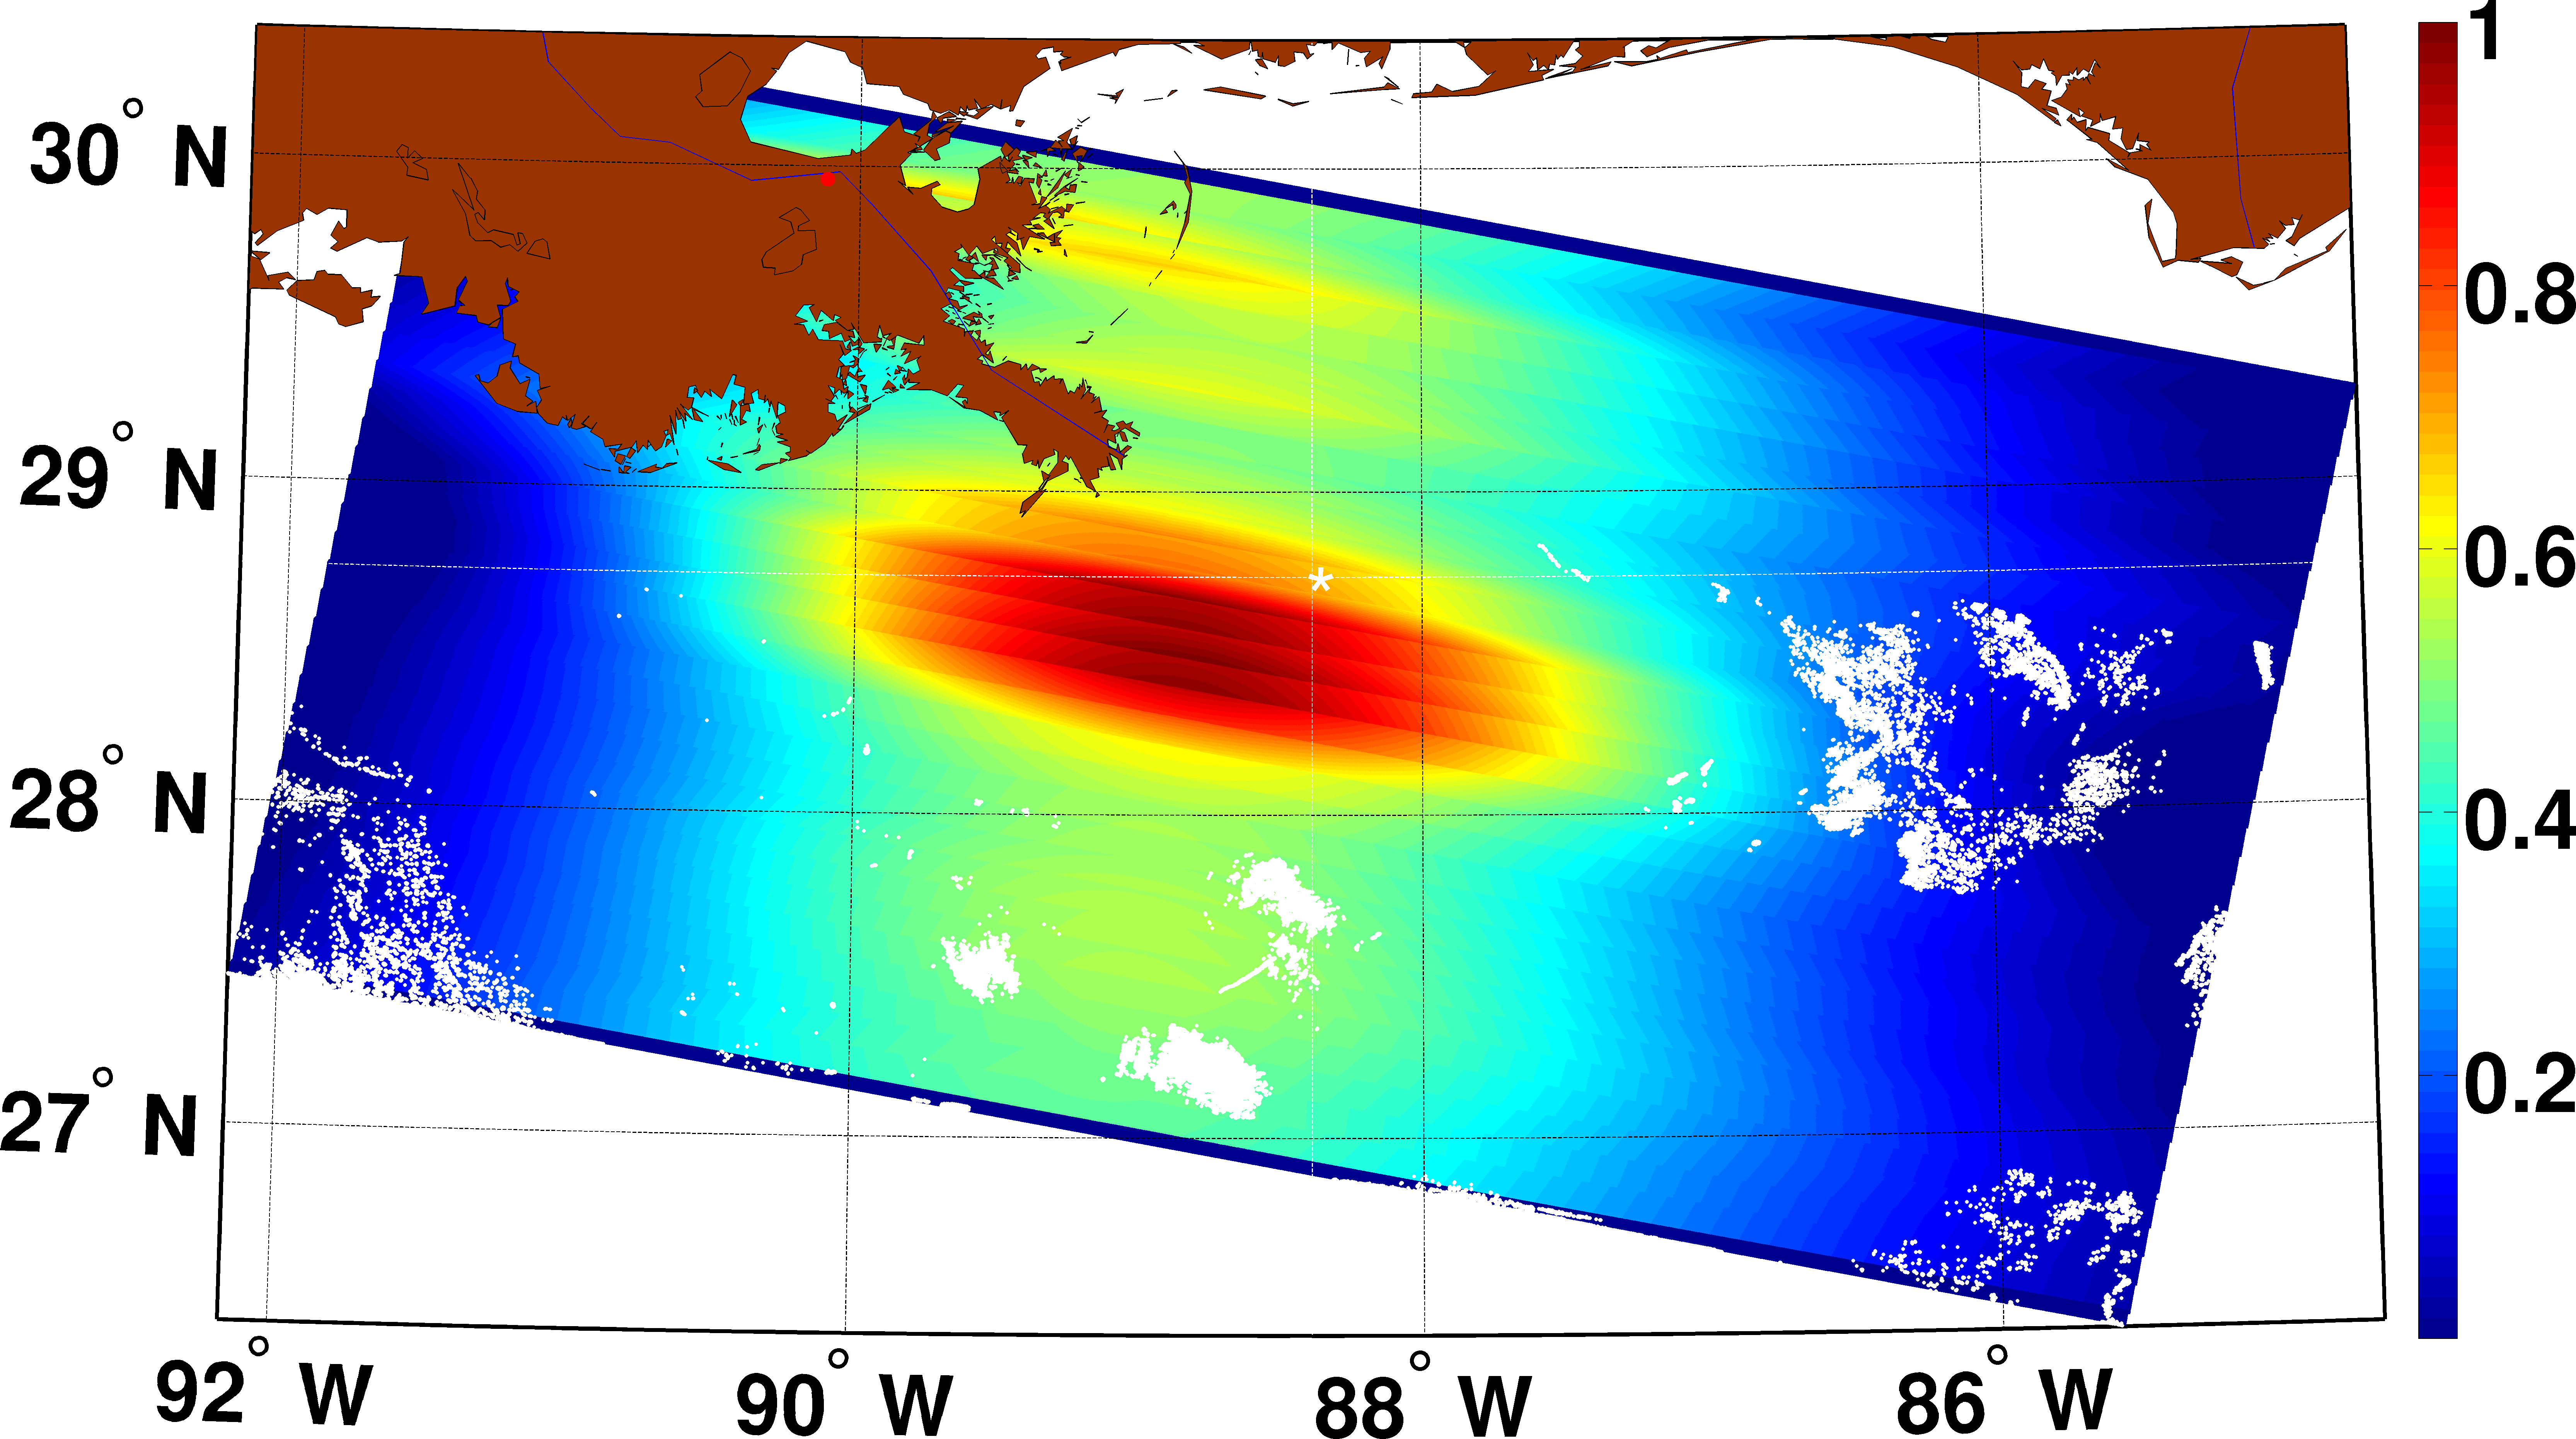
\includegraphics[width=1\linewidth]{fig2_4b}}
	\end{minipage}
	\\
	\begin{minipage}{.47\textwidth}
	    \subcaptionbox{\label{fig:2.4c}}
		{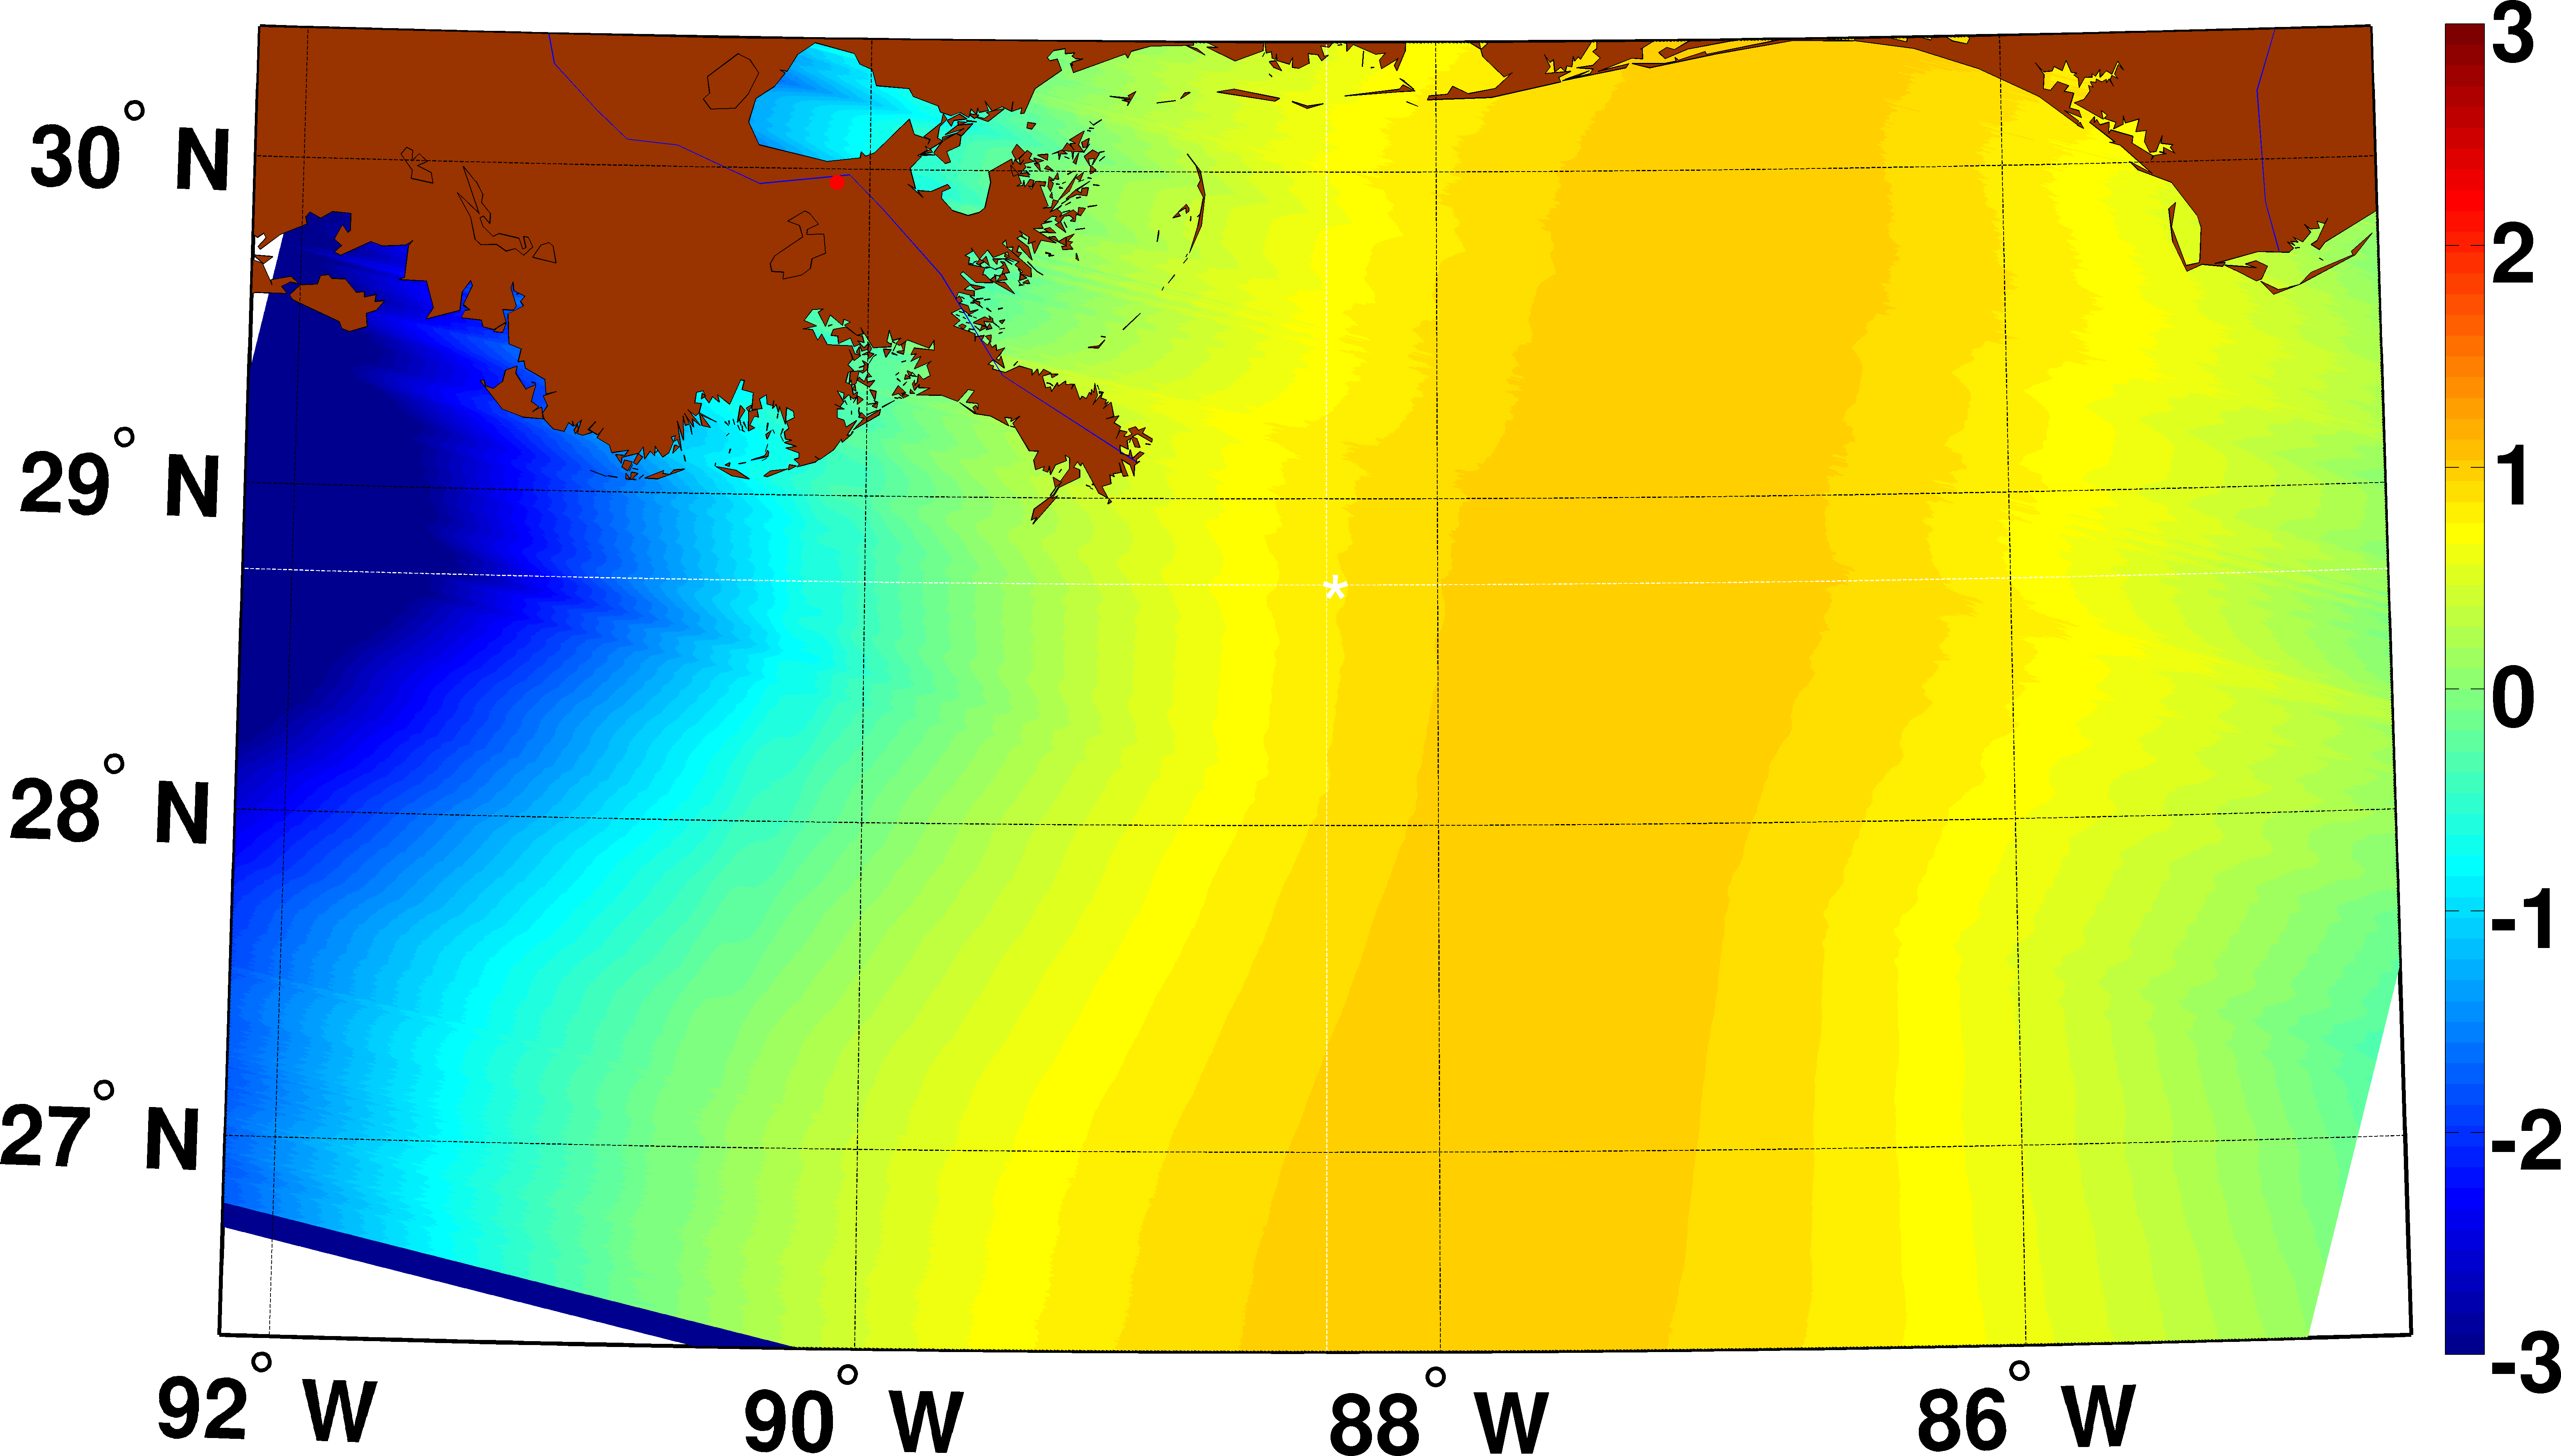
\includegraphics[width=1\linewidth]{fig2_4c}}
	\end{minipage}
	\hfill
	\begin{minipage}{.47\textwidth}
	    \subcaptionbox{\label{fig:2.4d}}
		{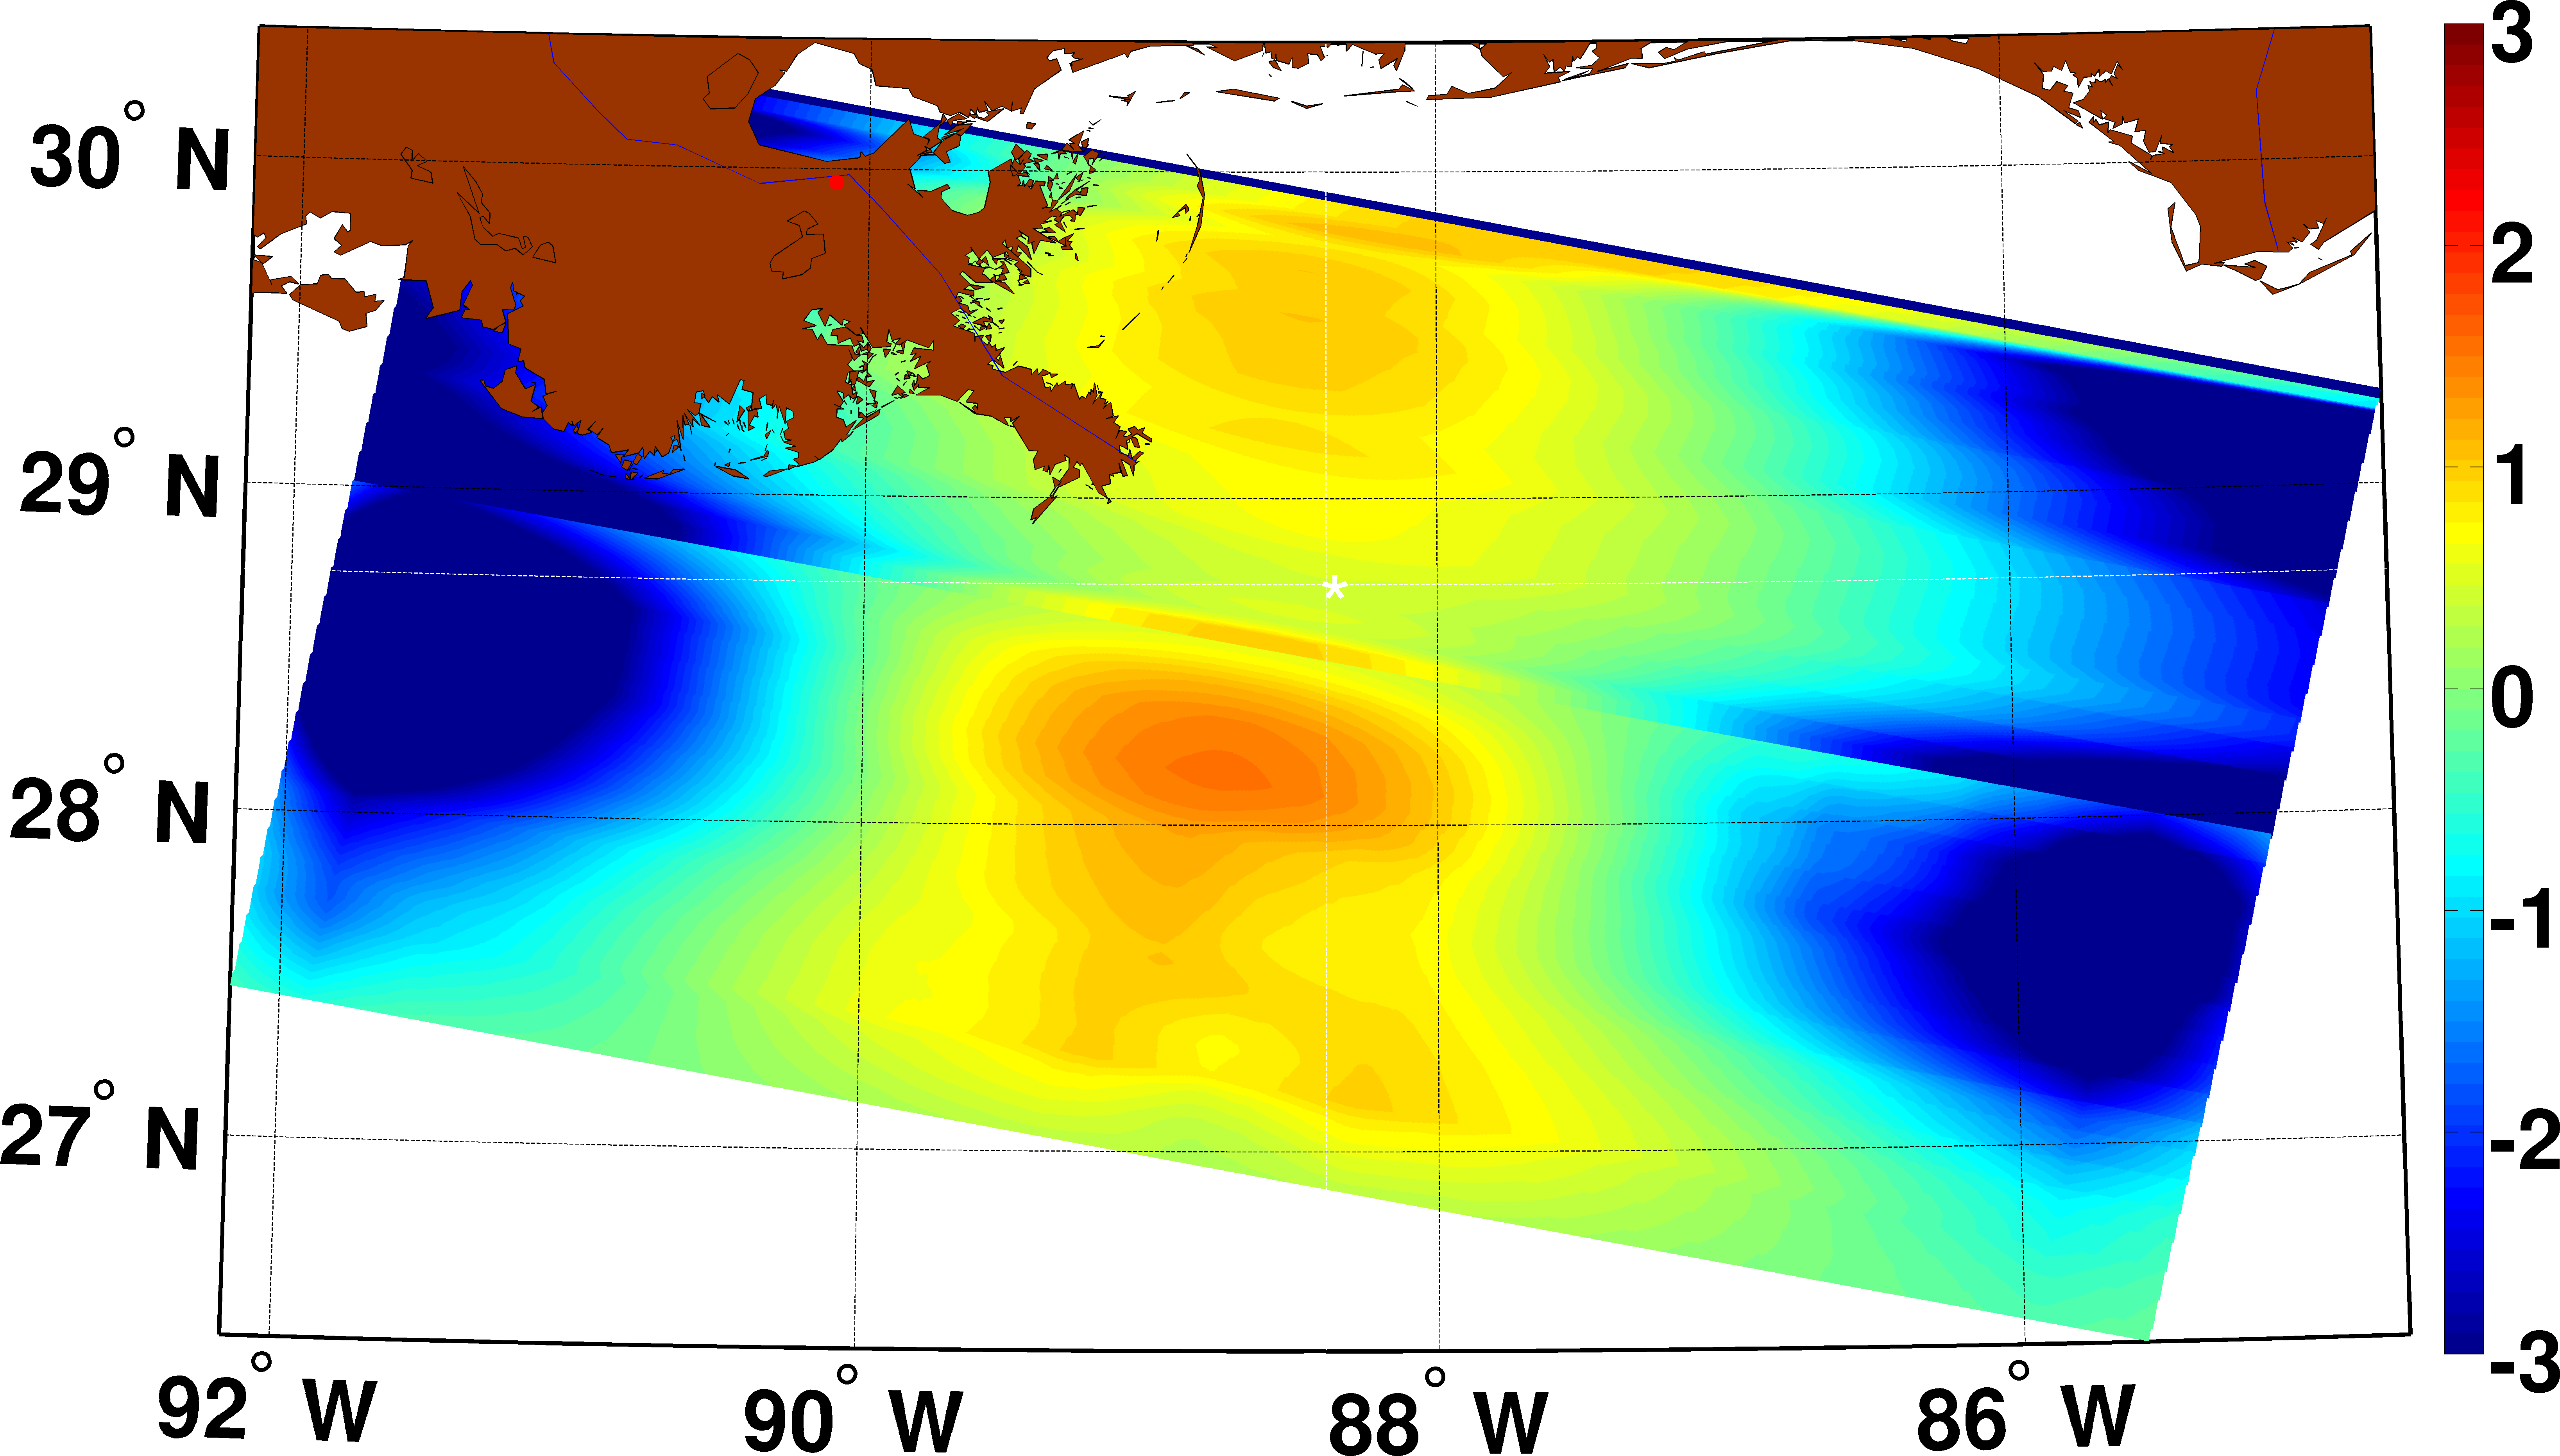
\includegraphics[width=1\linewidth]{fig2_4d}}
	\end{minipage}
    \\
    \floattitle{Усреднённая яркость $B_{0}$ изображений MERIS и MODIS (а) и (б), соответственно. Передаточная функция $T$, определяемая из уравнений \eqref{eq:1.15} для MERIS и \eqref{eq:1.7}, \eqref{eq:1.8} и \eqref{eq:1.9} для MODIS (в) и (г), соответственно. Наклонный линейный разрыв в поле $T$ (г) около 28.50${}^\circ$СШ появился в результате ``склеивания'' двух изображений MODIS/Terra, полученных в 16:45 и в 16:50 GMT}
    \caption{Усреднённая яркость $B_{0} $ с изображений MERIS и MODIS, а также передаточная функция $T$}
    \label{fig:2.4}
\end{figure}


Контрасты яркости солнечного блика $\tilde{B}/B_{0}$ для данных MERIS и MODIS представлены на Рисунке~\ref{fig:2.5}. Из представленного изображения видно, что поля контрастов согласуются, хотя есть и некоторые отличия. В районе 87${}^\circ$ЗД на обоих изображениях отчётливо видна ``нефтяная струя'', которая проявляется в виде светлых контрастов на изображении MERIS (Рисунок~\ref{fig:2.5a}), но в поле контрастов MODIS (Рисунок~\ref{fig:2.5b}) яркость струи меняется от светлой к тёмной. Если обратиться к Рисунку~\ref{fig:2.4b}, можно заметить, что передаточная функция $T$ меняет знак в этом районе, что соответствует зоне инверсии контрастов яркости. Нефтяная струя пересекает зону инверсии контрастов и, поэтому, контрасты яркости нефтяной струи в солнечном блике также меняет свой знак.



\begin{figure}[H]
   	\centering
	\begin{minipage}{.97\textwidth}
	    \subcaptionbox{\label{fig:2.5a}}
		{\includegraphics[width=1\linewidth]{fig2_5a}}
	\end{minipage}
	\hfill
	\\
	\begin{minipage}{.97\textwidth}
	    \subcaptionbox{\label{fig:2.5b}}
		{\includegraphics[width=1\linewidth]{fig2_5b}}
	\end{minipage}
    \\
    \floattitle{Проявление нефтяного разлива в контрастах яркости солнечного блика $\tilde{B}/B_{0}$, на изображениях MERIS (а) и MODIS (б)}
    \caption{Контрасты яркости солнечного блика $\tilde{B}/B_{0}$}
    \label{fig:2.5}
\end{figure}


На Рисунке~\ref{fig:2.6} приведены контрасты СКН $\tilde{s}^{2} /s_{0}^{2}$, полученные по изображениям яркости в солнечном блике MERIS и MODIS (Рисунок~\ref{fig:2.5}), с использованием передаточной функции, представленной на Рисунке~\ref{fig:2.4}. Сопоставляя полученные изображения, видно, что аномалии СКН, полученные с применением двух различных алгоритмов (см. выражения \eqref{eq:1.7} и \eqref{eq:1.15} в разделах \ref{sec:1.3.2} и \ref{sec:1.3.3}) к двум независимым изображениям, дают очень схожие результаты. Это подтверждает надежность предложенной методологии. Усреднённые контрасты СКН в нефтяной струе, полученные по изображениям MODIS и MERIS, показаны на Рисунке~\ref{fig:2.2} (справа).

Стоит также отметить несколько особенностей, наблюдаемых на обработанных изображениях (см. Рисунок~\ref{fig:2.6}). Во-первых, линейные особенности (отмеченные красными стрелками), с сингулярным поведением контрастов СКН, связаны с зонами инверсии контрастов. Также на изображениях наблюдаются отрицательные и положительные вариаций контрастов в области, заключённой в жёлтый контур, близ устья реки Миссисипи. Более того, эти положительные/отрицательные значения на обоих изображениях не перекрываются. Учитывая тот факт, что нефтяная плёнка подавляет короткие волны и СКН, ``яркие'' особенности СКН на Рисунке~\ref{fig:2.6} должны рассматриваться как артефакты, вызванные какими-то другими факторами. Если предположить, что толщина нефтяной плёнки в этом районе значительно больше длины волны красного света (640-680\textit{нм}), т.е. толщина порядка 1 микрона и более, то в этом случае, оптические свойства самой нефти могут доминировать над изменениями яркости морской поверхности в зоне, покрытой этой нефтью. Предложенный алгоритм не учитывает возможность изменения ``цвета'' поверхности, поэтому смена знака и изменение амплитуды восстановленных контрастов некорректны и не несут физического смысла.

Чтобы подробнее продемонстрировать эффект изменения толщины нефтяной плёнки, рассмотрим случай синхронной съёмки приборами MERIS и ENVISAT ASAR. На Рисунке~\ref{fig:2.7} представлены восстановленная по данным РСА скорость ветра (с использованием алгоритма CMOD-4) и яркость морской поверхности в красном канале MERIS над Мексиканским заливом 26 Апреля 2010. Нефтяной разлив виден на обоих изображениях. Увеличенные фрагменты этих изображений представлены для контрастов УЭПР и контрастов СКН на Рисунке~\ref{fig:2.8}. Контрасты СКН получены при помощи метода, описанного в Главе~\ref{chap:1}.



\begin{figure}[H]
   	\centering
	\begin{minipage}{.83\textwidth}
	    \subcaptionbox{\label{fig:2.6a}}
		{\includegraphics[width=1\linewidth]{fig2_6a}}
	\end{minipage}
	\hfill
	\\
	\begin{minipage}{.83\textwidth}
	    \subcaptionbox{\label{fig:2.6b}}
		{\includegraphics[width=1\linewidth]{fig2_6b}}
	\end{minipage}
    \\
    \floattitle{Красными стрелками обозначены области инверсии контрастов, где восстановленный СКН имеет сингулярные значения и не несёт физического смысла. Яркие участки контрастов СКН, обведённые жёлтым контуром, не относятся к особенностям шероховатости морской поверхности, но, скорее всего, являются индикаторами проявления оптических свойств нефтяной плёнки. Таким образом, толщина нефтяной плёнки в этой области (внутри контура) может быть значительно большей длины волны красного света}
    \caption{Аномалии СКН $\widetilde{s^{2} }/s^{2}$, восстановленные по данным прибора MERIS (а) и MODIS (б)}
    \label{fig:2.6}
\end{figure}


\begin{figure}[H]
   	\centering
	\begin{minipage}{.49\textwidth}
	    \subcaptionbox{\label{fig:2.7a}}
		{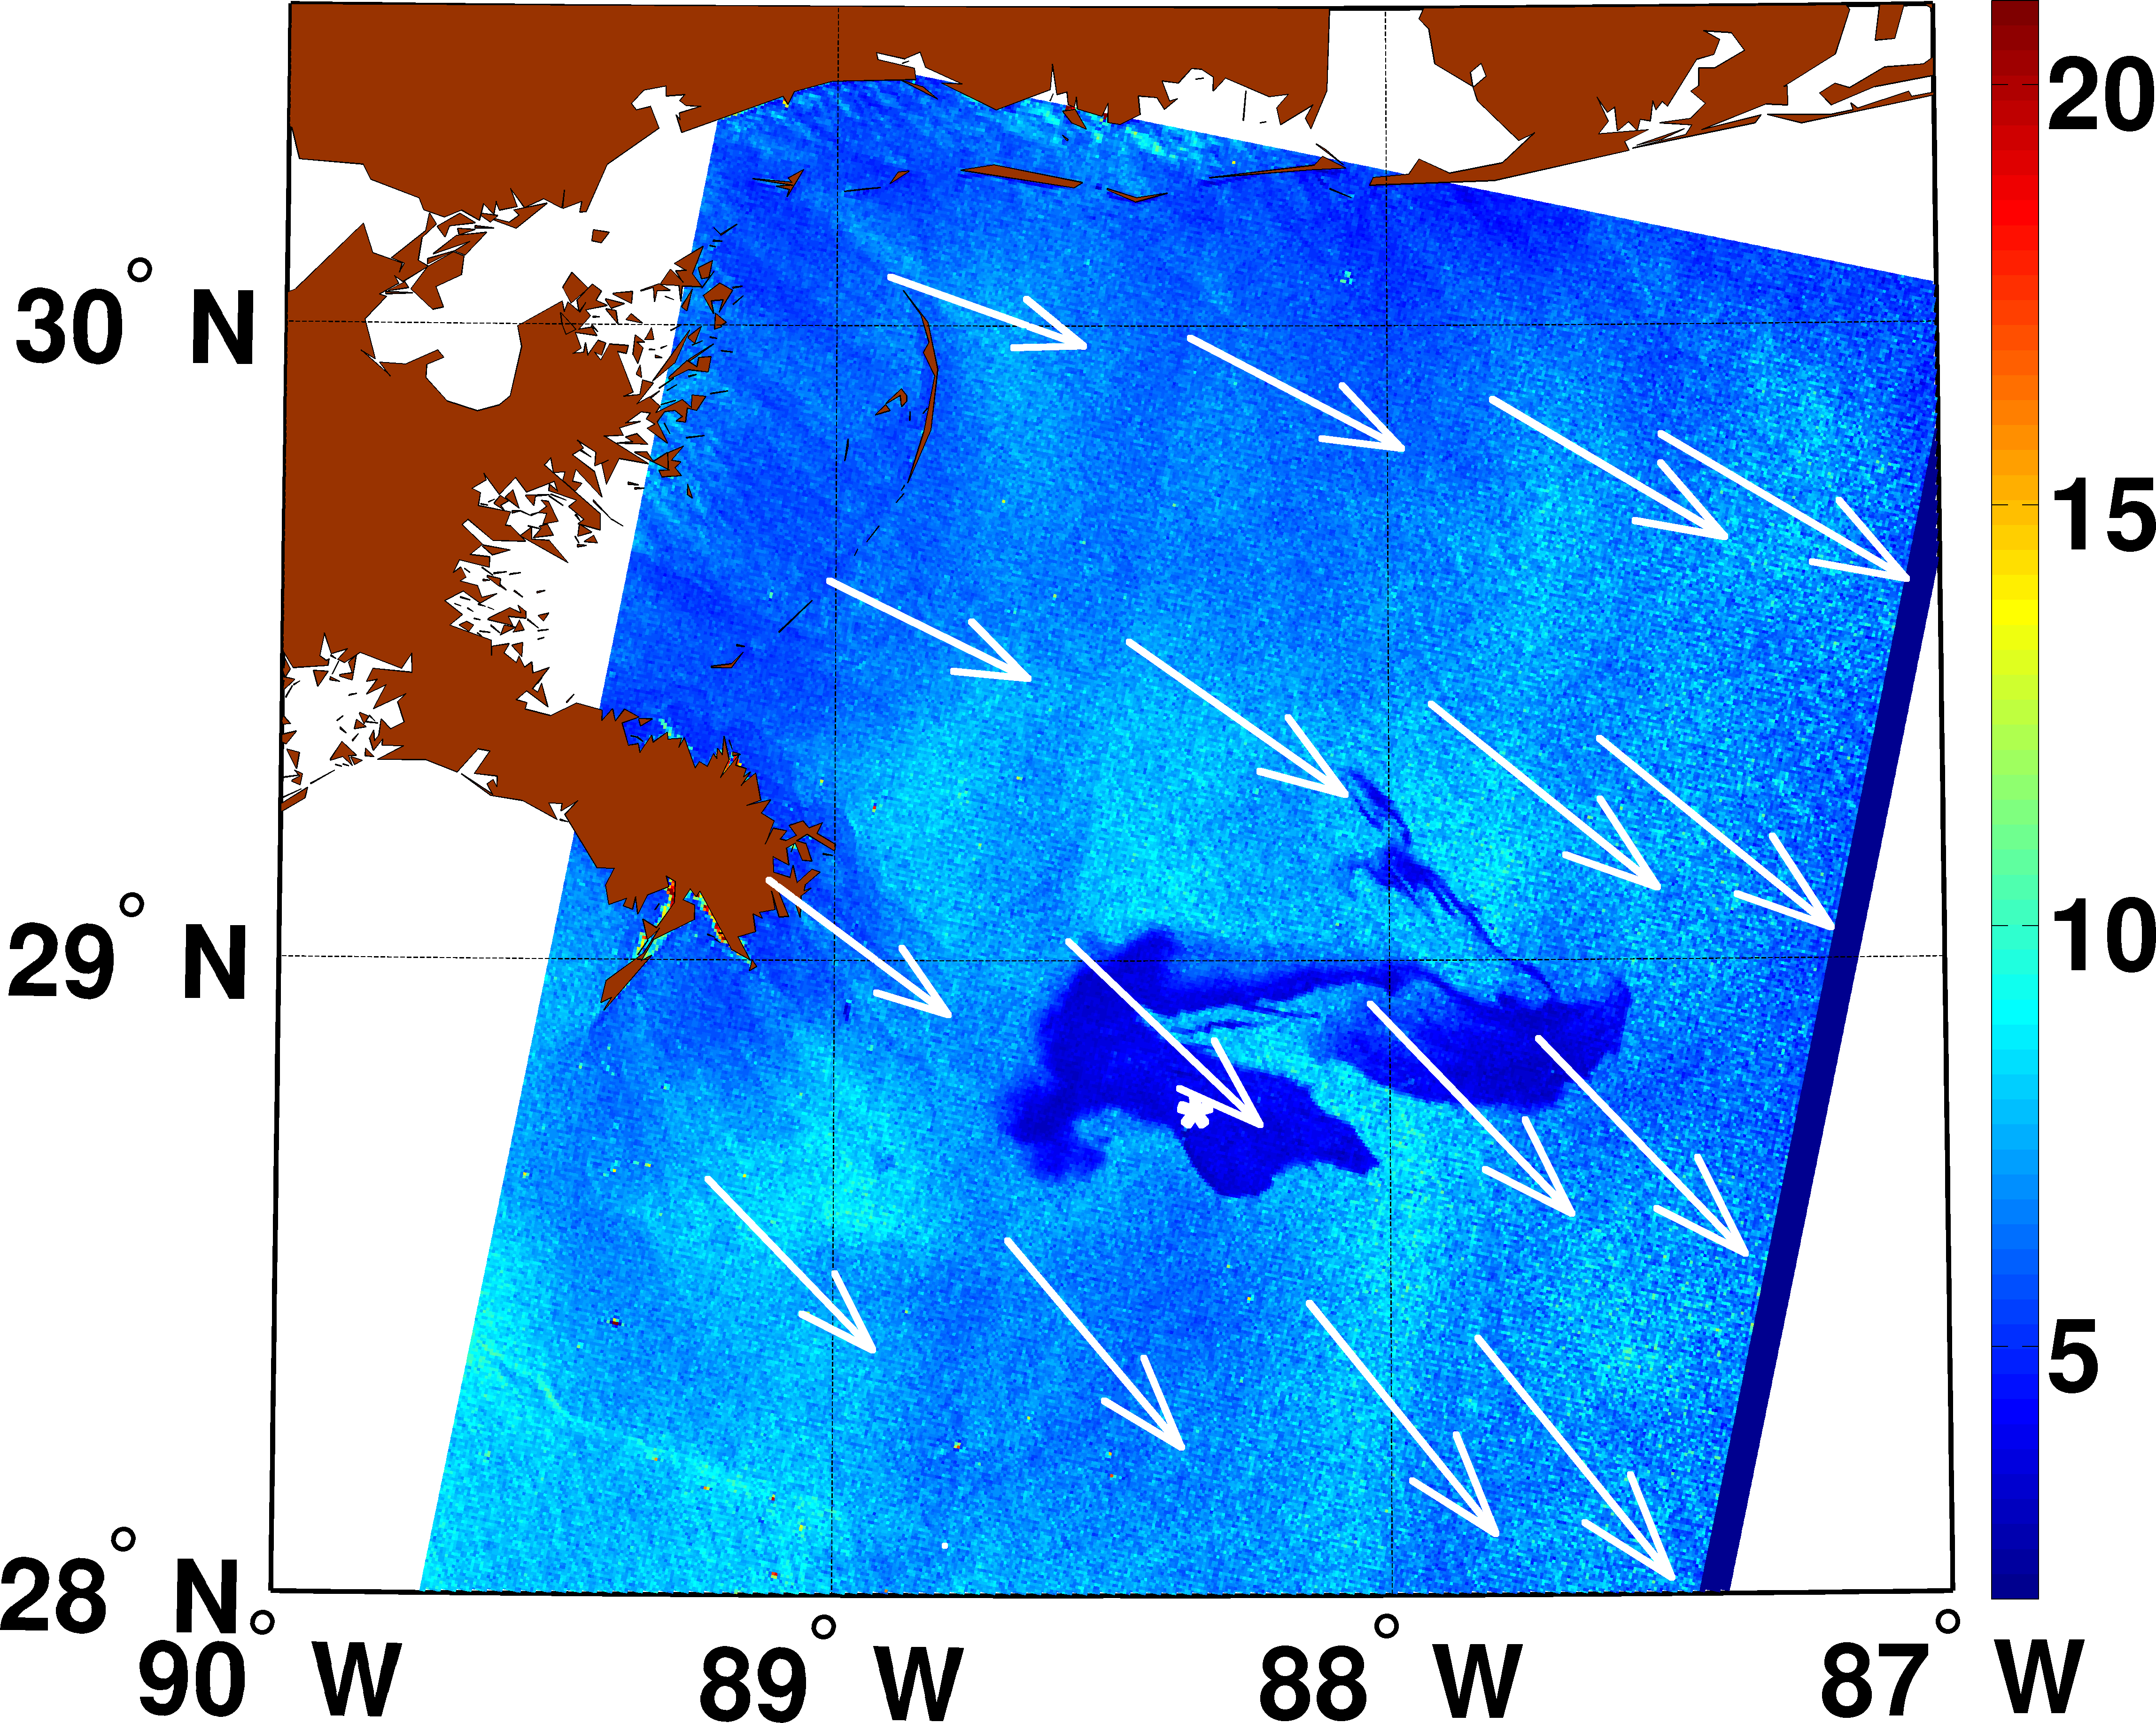
\includegraphics[width=1\linewidth]{fig2_7a}}
	\end{minipage}
	\hfill
	\begin{minipage}{.49\textwidth}
	    \subcaptionbox{\label{fig:2.7b}}
		{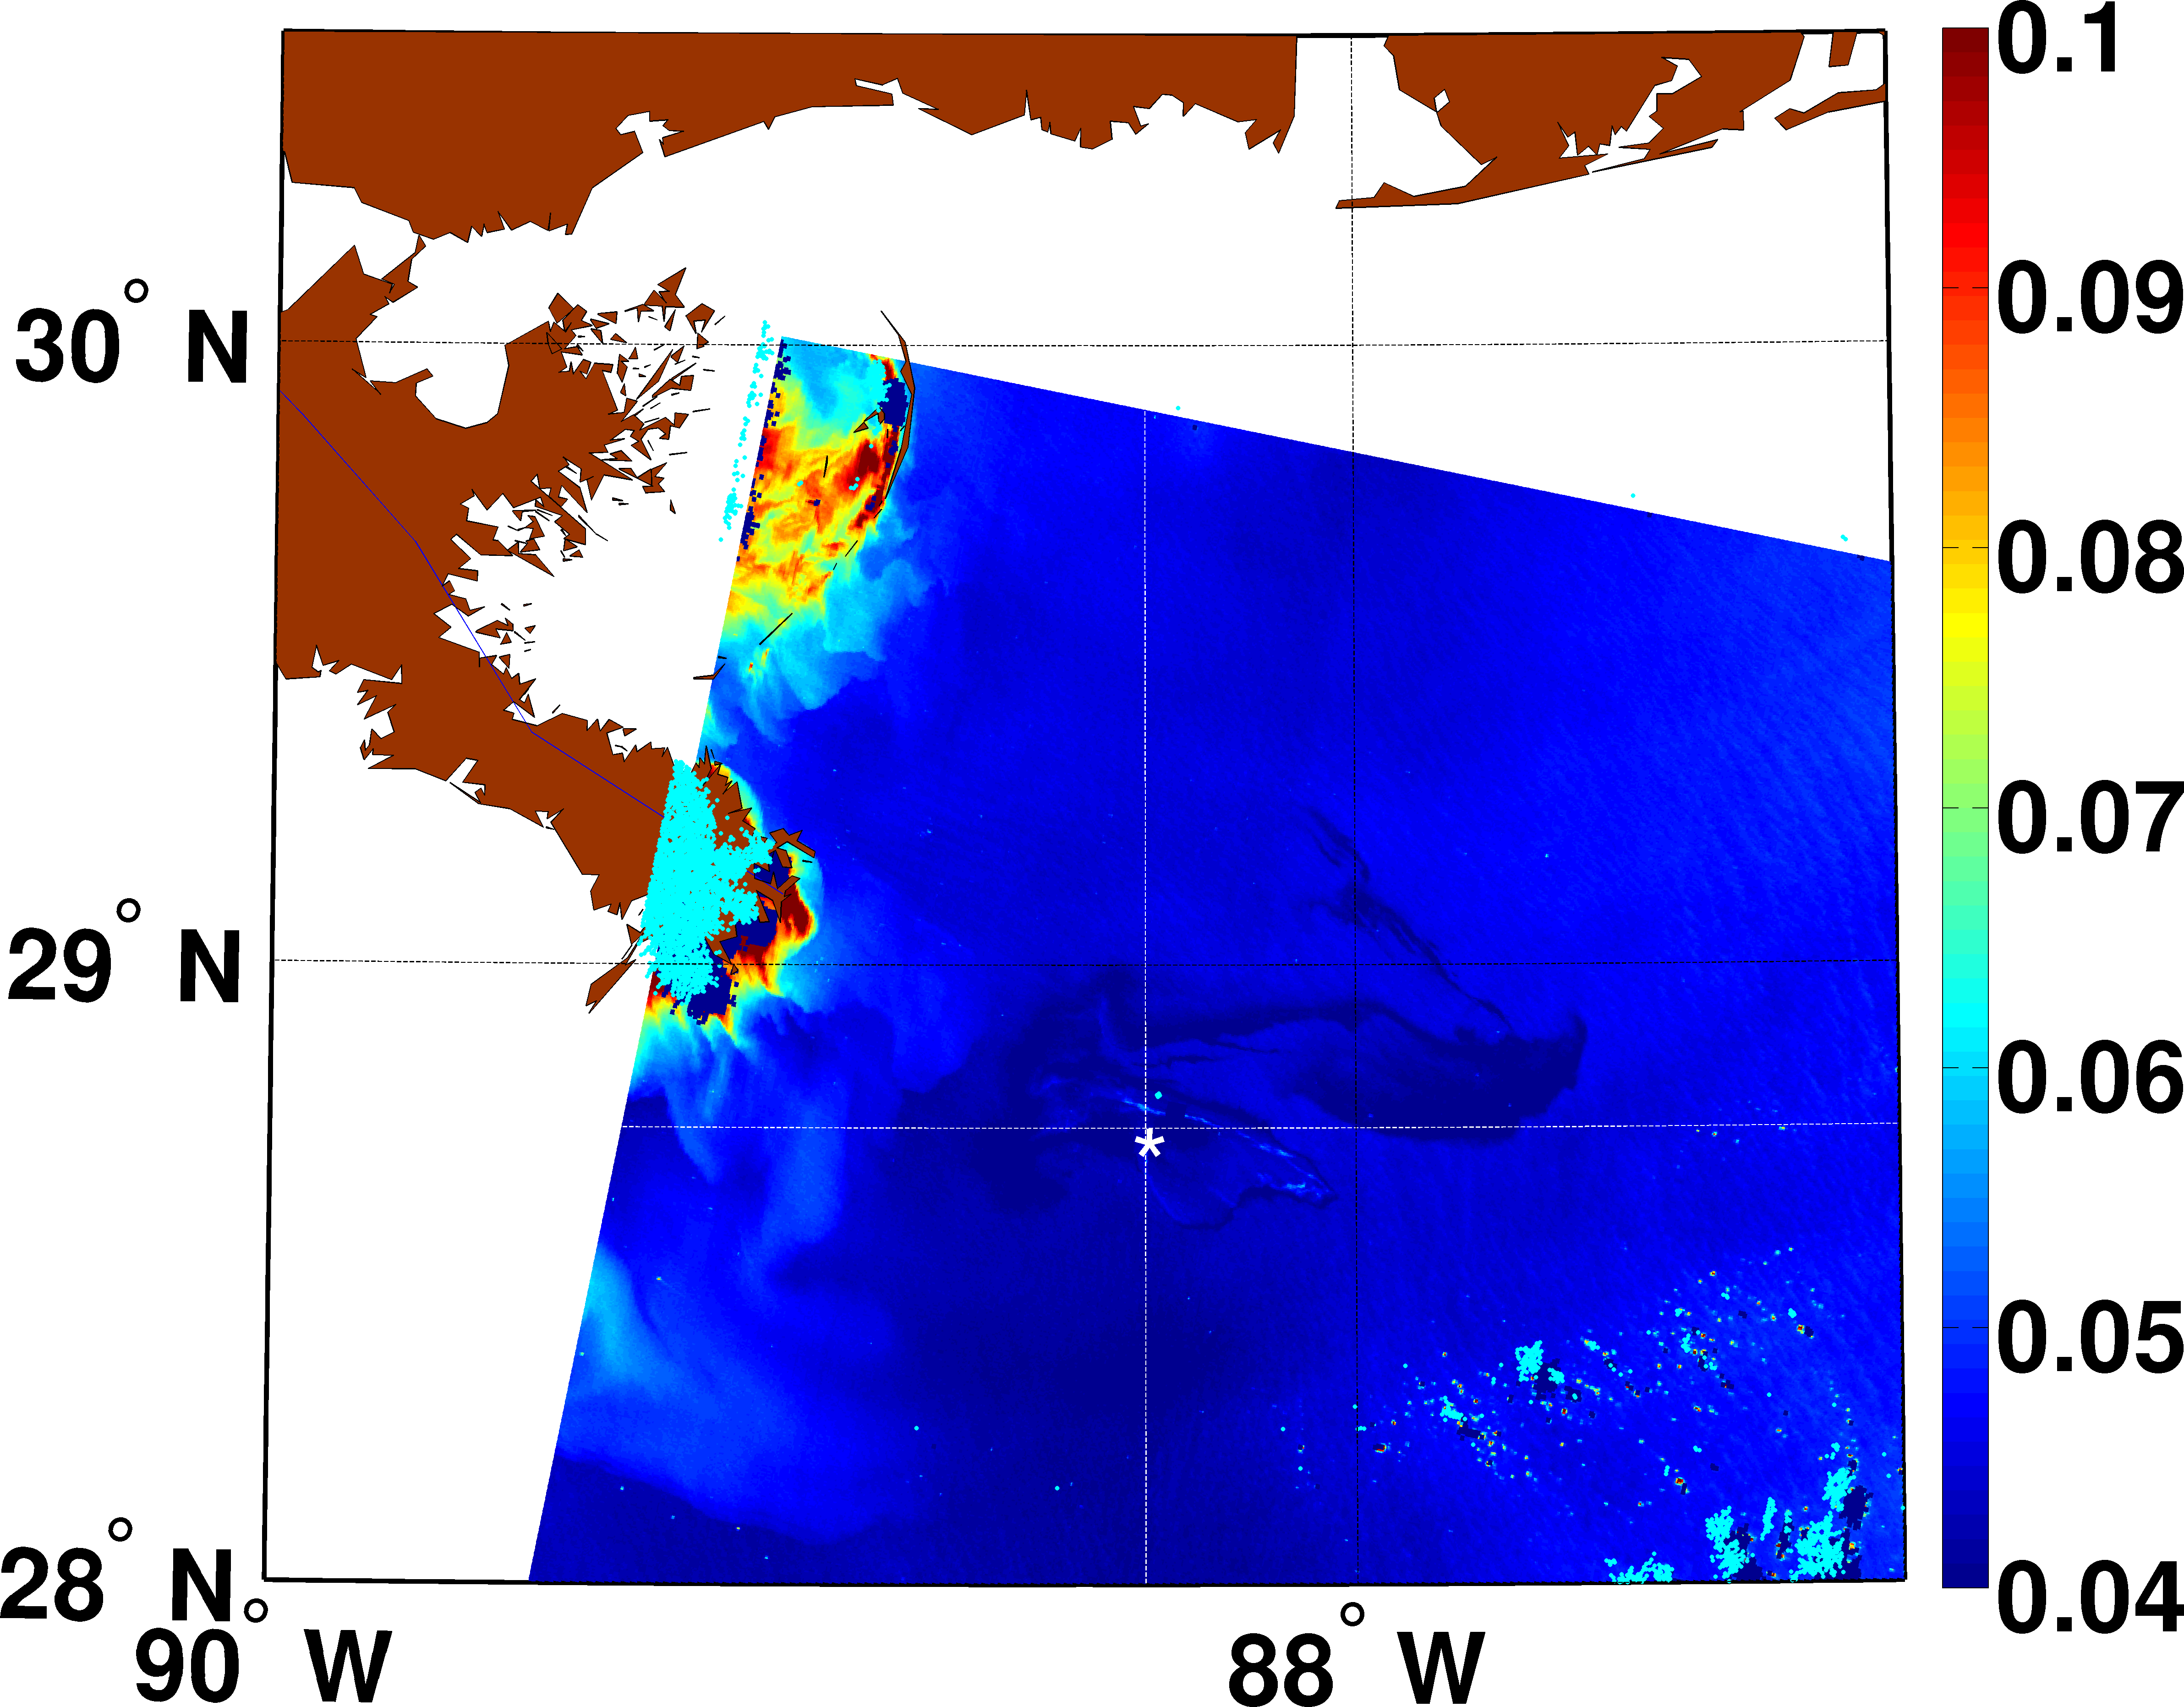
\includegraphics[width=1\linewidth]{fig2_7b}}
	\end{minipage}
    \\
    \floattitle{На изображении MERIS видно проявление нефтяного разлива в Мексиканском заливе в красном канале 26 Апреля 2010г. ASAR представлено в виде скорости ветра, рассчитанной по УЭПР с использованием модели CMOD-4. Белые стрелки на РСА изображении показывают направление ветра NCEP}
    \caption{Изображения (а) ASAR (15:58 GMT), и (б) MERIS (15:56 GMT)}
    \label{fig:2.7}
\end{figure}


Из Рисунка~\ref{fig:2.7} видно, что нефтяной разлив на обоих изображениях имеет схожую ``геометрию'', однако, контрасты УЭПР и СКН значительно разнятся. Разделим области, изображённого на Рисунке~\ref{fig:2.8} разлива, на 2 части -- внутри и вне жёлтого контура. Поля контрастов СКН и УЭПР ``вне'' жёлтого контура визуально хорошо коррелируют. Связь контрастов СКН и УЭПР представлена на Рисунке~\ref{fig:2.9}. Из Рисунка~\ref{fig:2.9} видно, что контрасты СКН хорошо коррелируют с УЭПР, а значения СКН несколько ниже УЭПР с коэффициентом отношения около 0.6: $\tilde{s}^{2} /s^{2} \approx 0.6\cdot \tilde{\sigma }_{0} /\sigma _{0}$.

Контрасты СКН, усреднённые по части изображения MERIS ``вне'' жёлтого контура также приводятся на Рисунке~\ref{fig:2.2} (справа). Отметим, что тот же слик также наблюдался прибором MODIS получасом позднее, однако, здесь это изображение не приводится. Обработка этого спутникового снимка показало, что поле контрастов СКН, представленное на Рисунке~\ref{fig:2.8a}, очень схоже на усреднённые значения контрастов СКН по данным MODIS на Рисунке~\ref{fig:2.2} (справа).

Усреднённые контрасты УЭПР нефтяного слика ``вне'' жёлтого контура из Рисунка~\ref{fig:2.8b} приведены на Рисунке~\ref{fig:2.9} (справа). Две другие оценки контрастов УЭПР на Рисунке~\ref{fig:2.9} (справа) получены при меньших скоростях ветра по данным РСА ASAR 25 Мая 2010, 15:47 GMT на следующий день после получения обсуждаемых изображений MERIS и MODIS на Рисунке~\ref{fig:2.3}. В обоих случаях, скорость ветра была восстановлена по изображениям ASAR с использованием алгоритма CMOD-4 (см., например, Рисунок~\ref{fig:2.7a}). Представленные на Рисунке~\ref{fig:2.9} контрасты УЭПР, показывают их сильную зависимость от скорости ветра. Сопоставляя контрасты УЭПР на Рисунке~\ref{fig:2.9} (справа) и контрасты СКН на Рисунке~\ref{fig:2.2} (справа) можно заключить, что при слабых и умеренных скоростях ветра, нефтяные слики проявляются на РСА изображениях лучше, нежели на оптических.



\begin{figure}[!ht]
   	\centering
	\begin{minipage}{.49\textwidth}
	    \subcaptionbox{\label{fig:2.8a}}
		{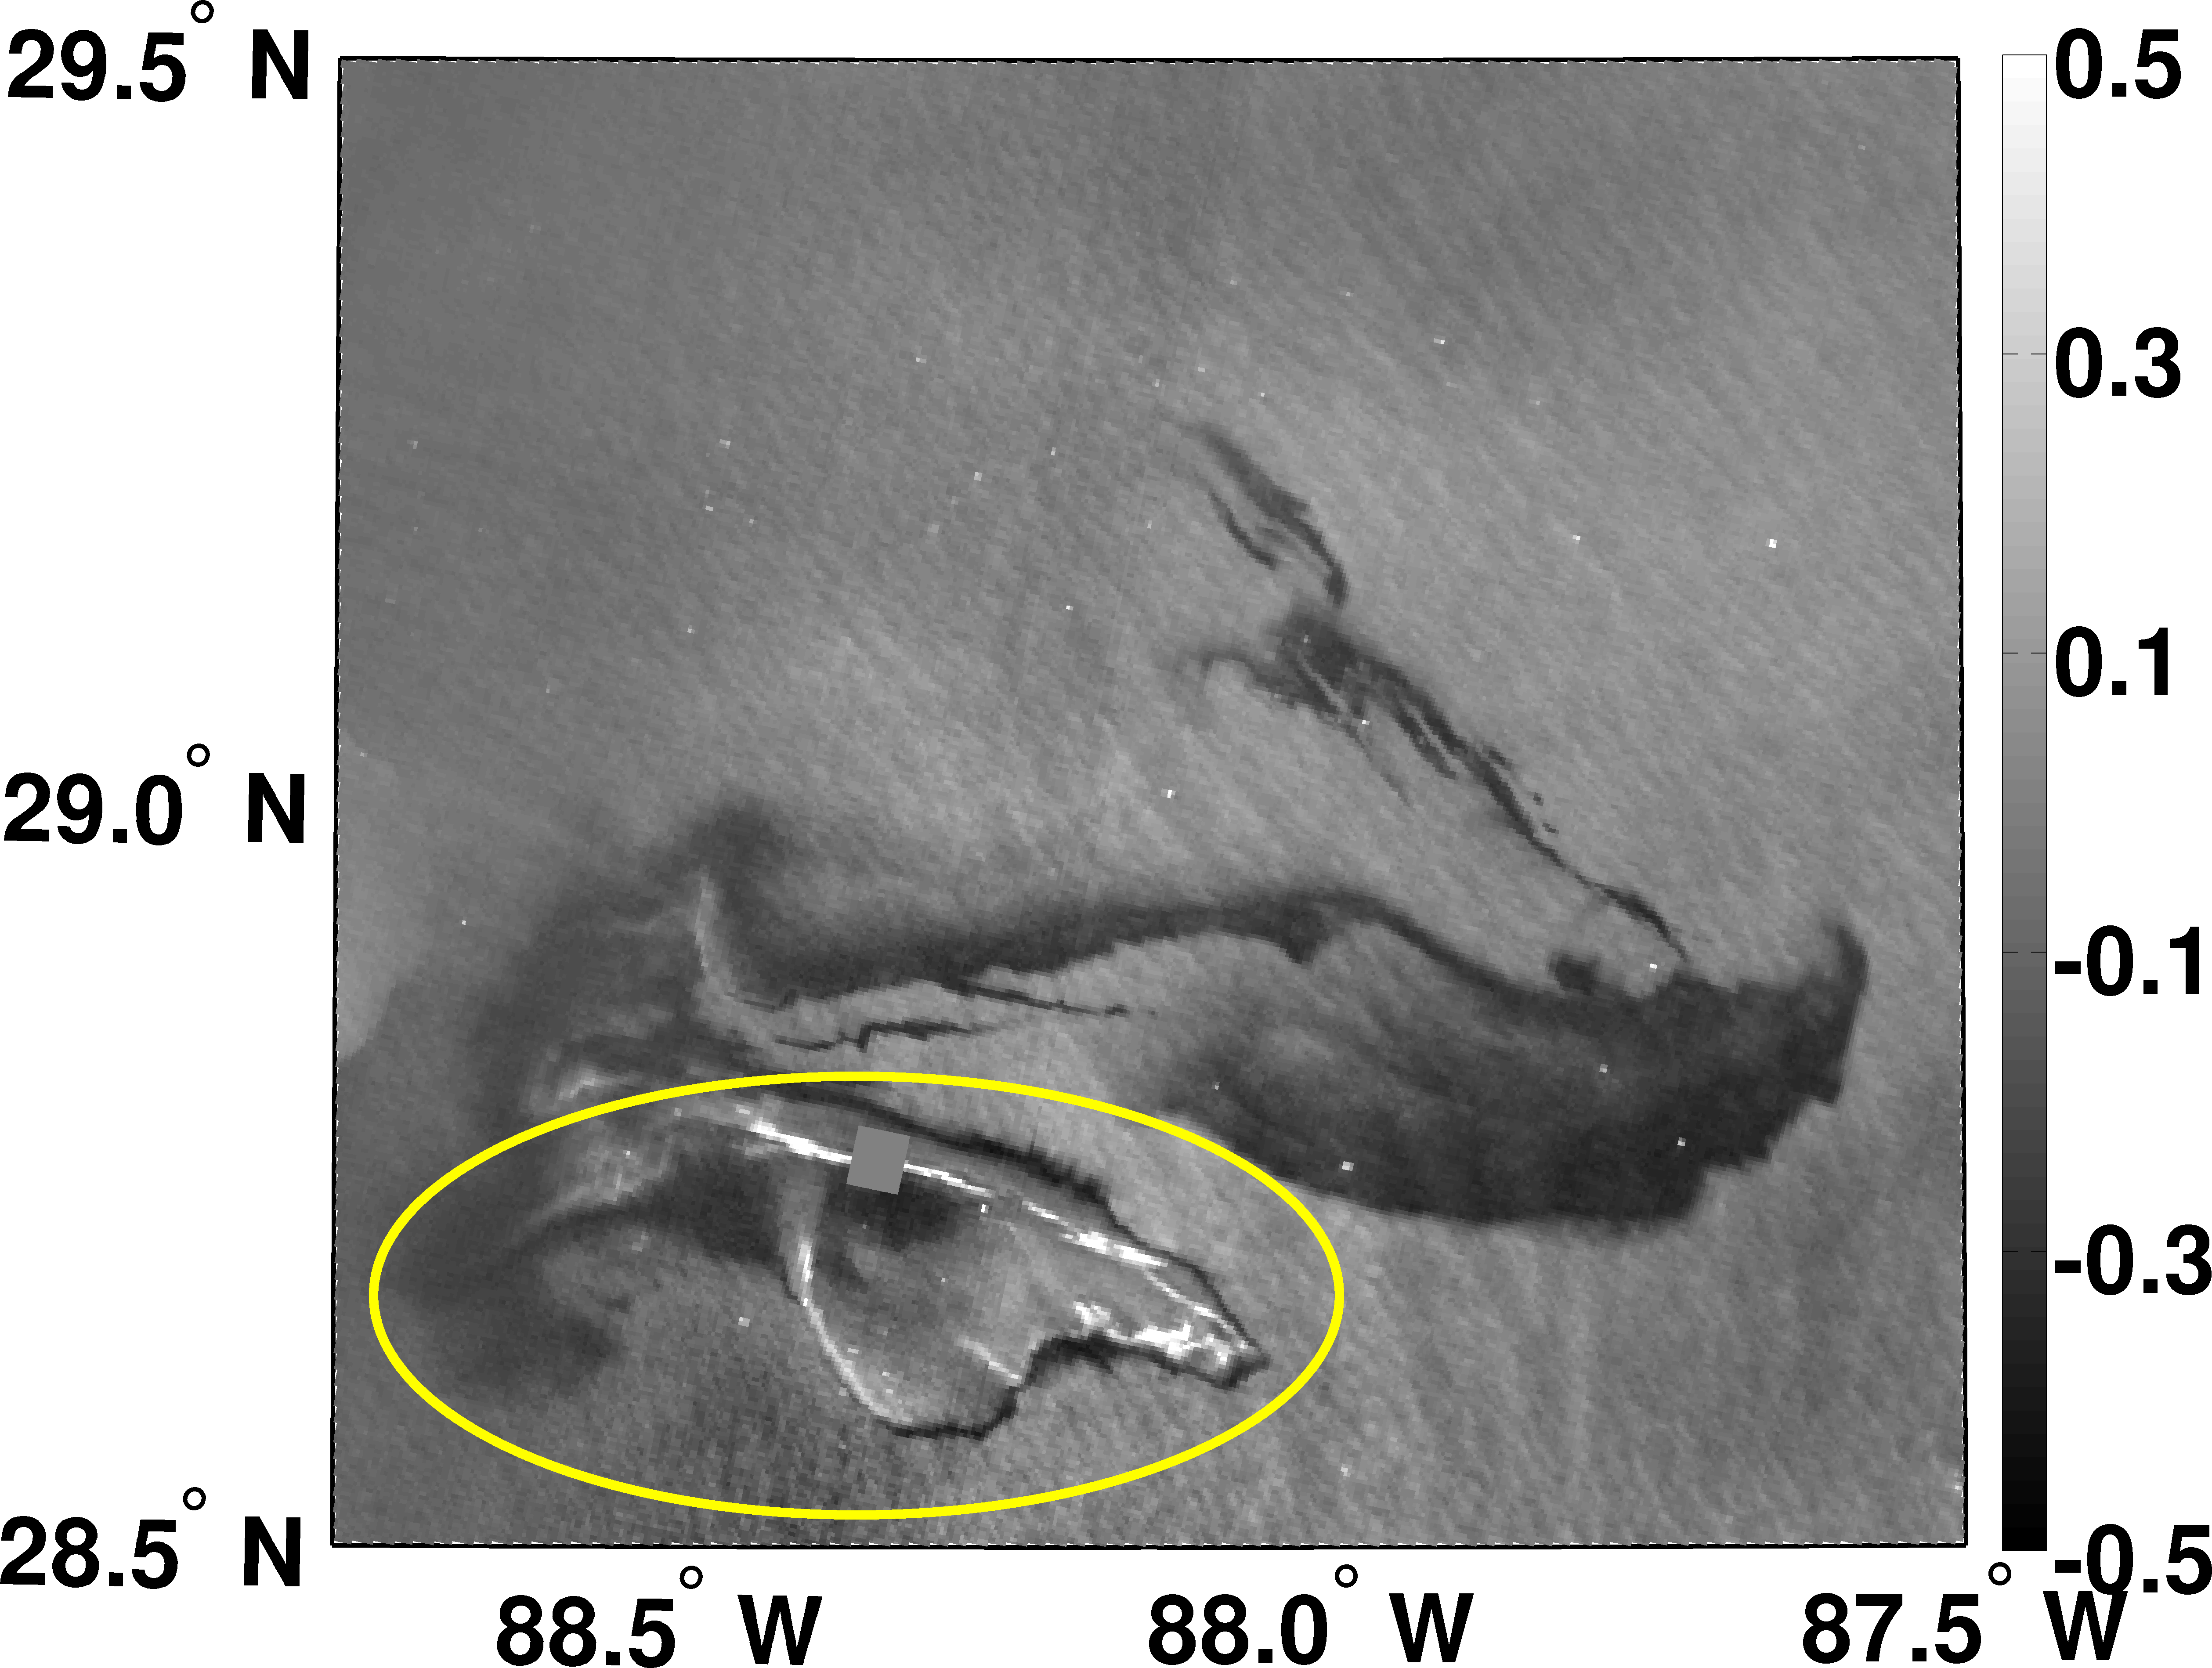
\includegraphics[width=1\linewidth]{fig2_8a}}
	\end{minipage}
	\hfill
	\begin{minipage}{.49\textwidth}
	    \subcaptionbox{\label{fig:2.8b}}
		{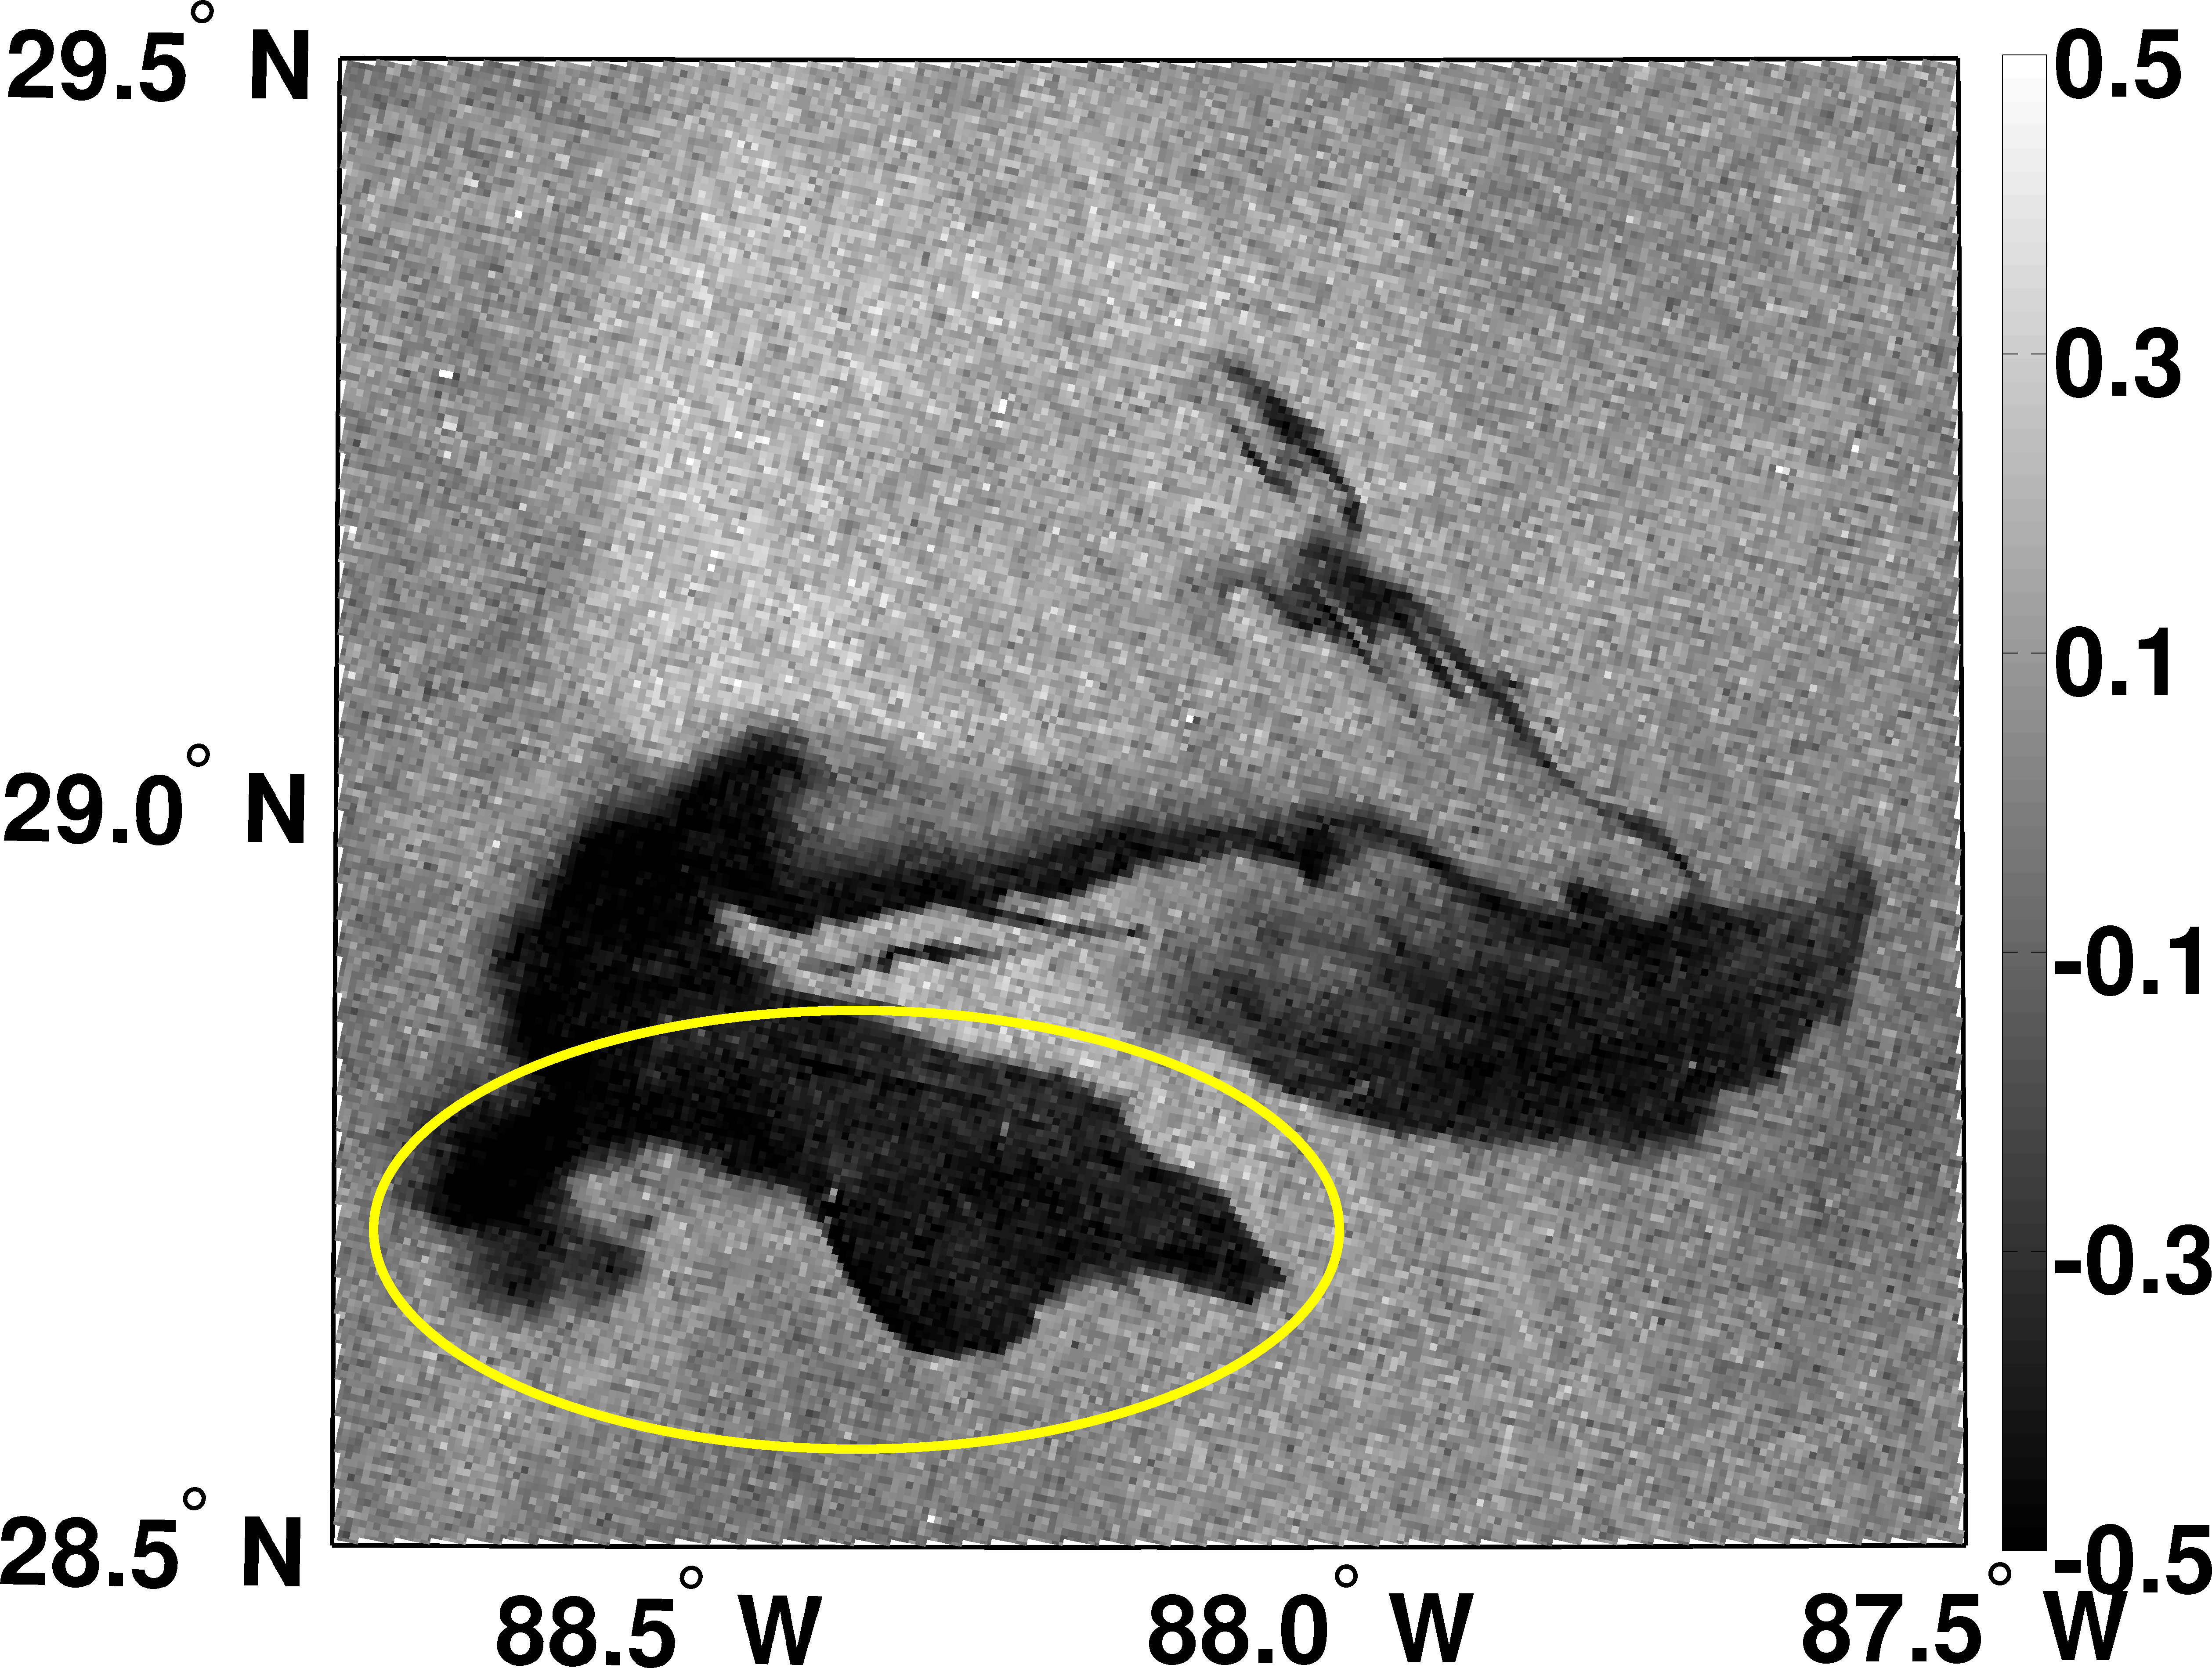
\includegraphics[width=1\linewidth]{fig2_8b}}
	\end{minipage}
    \\
    \floattitle{Изображения содержат нефтяной разлив и представлены в терминах УЭПР (линейные единицы) и контрастов СКН. Толщина нефтяной плёнки в области внутри жёлтого контура значительно больше длины волны красного света}
    \caption{Увеличенные фрагменты изображений MERIS (а) и ASAR (б), представленных на Рисунке~\ref{fig:2.7}}
    \label{fig:2.8}
\end{figure}


Возвращаясь к Рисунку~\ref{fig:2.8}, отметим, что область внутри жёлтого контура демонстрирует аномальное поведение контрастов УЭПР. Контрасты УЭПР в этой области обладают сильной изменчивостью, и некоторые из участков проявляются очень ярко. Исходя из данных РСА видно, что короткое ветровое волнение значительно подавляется в этой области. Поэтому можно предположить, что яркие участки контрастов СКН внутри жёлтого контура не связаны с усилением шероховатости морской поверхности, а, скорее всего, являются следствием проявления оптических свойств нефтяной плёнки, если толщина нефтяной плёнки значительно больше длины волны красного света. Таким образом, можно предположить, что ``яркие особенности'', хорошо различимые в поле контрастов СКН внутри жёлтого контура, относятся к цвету самой нефти.



\begin{figure}[!ht]
   	\centering
	{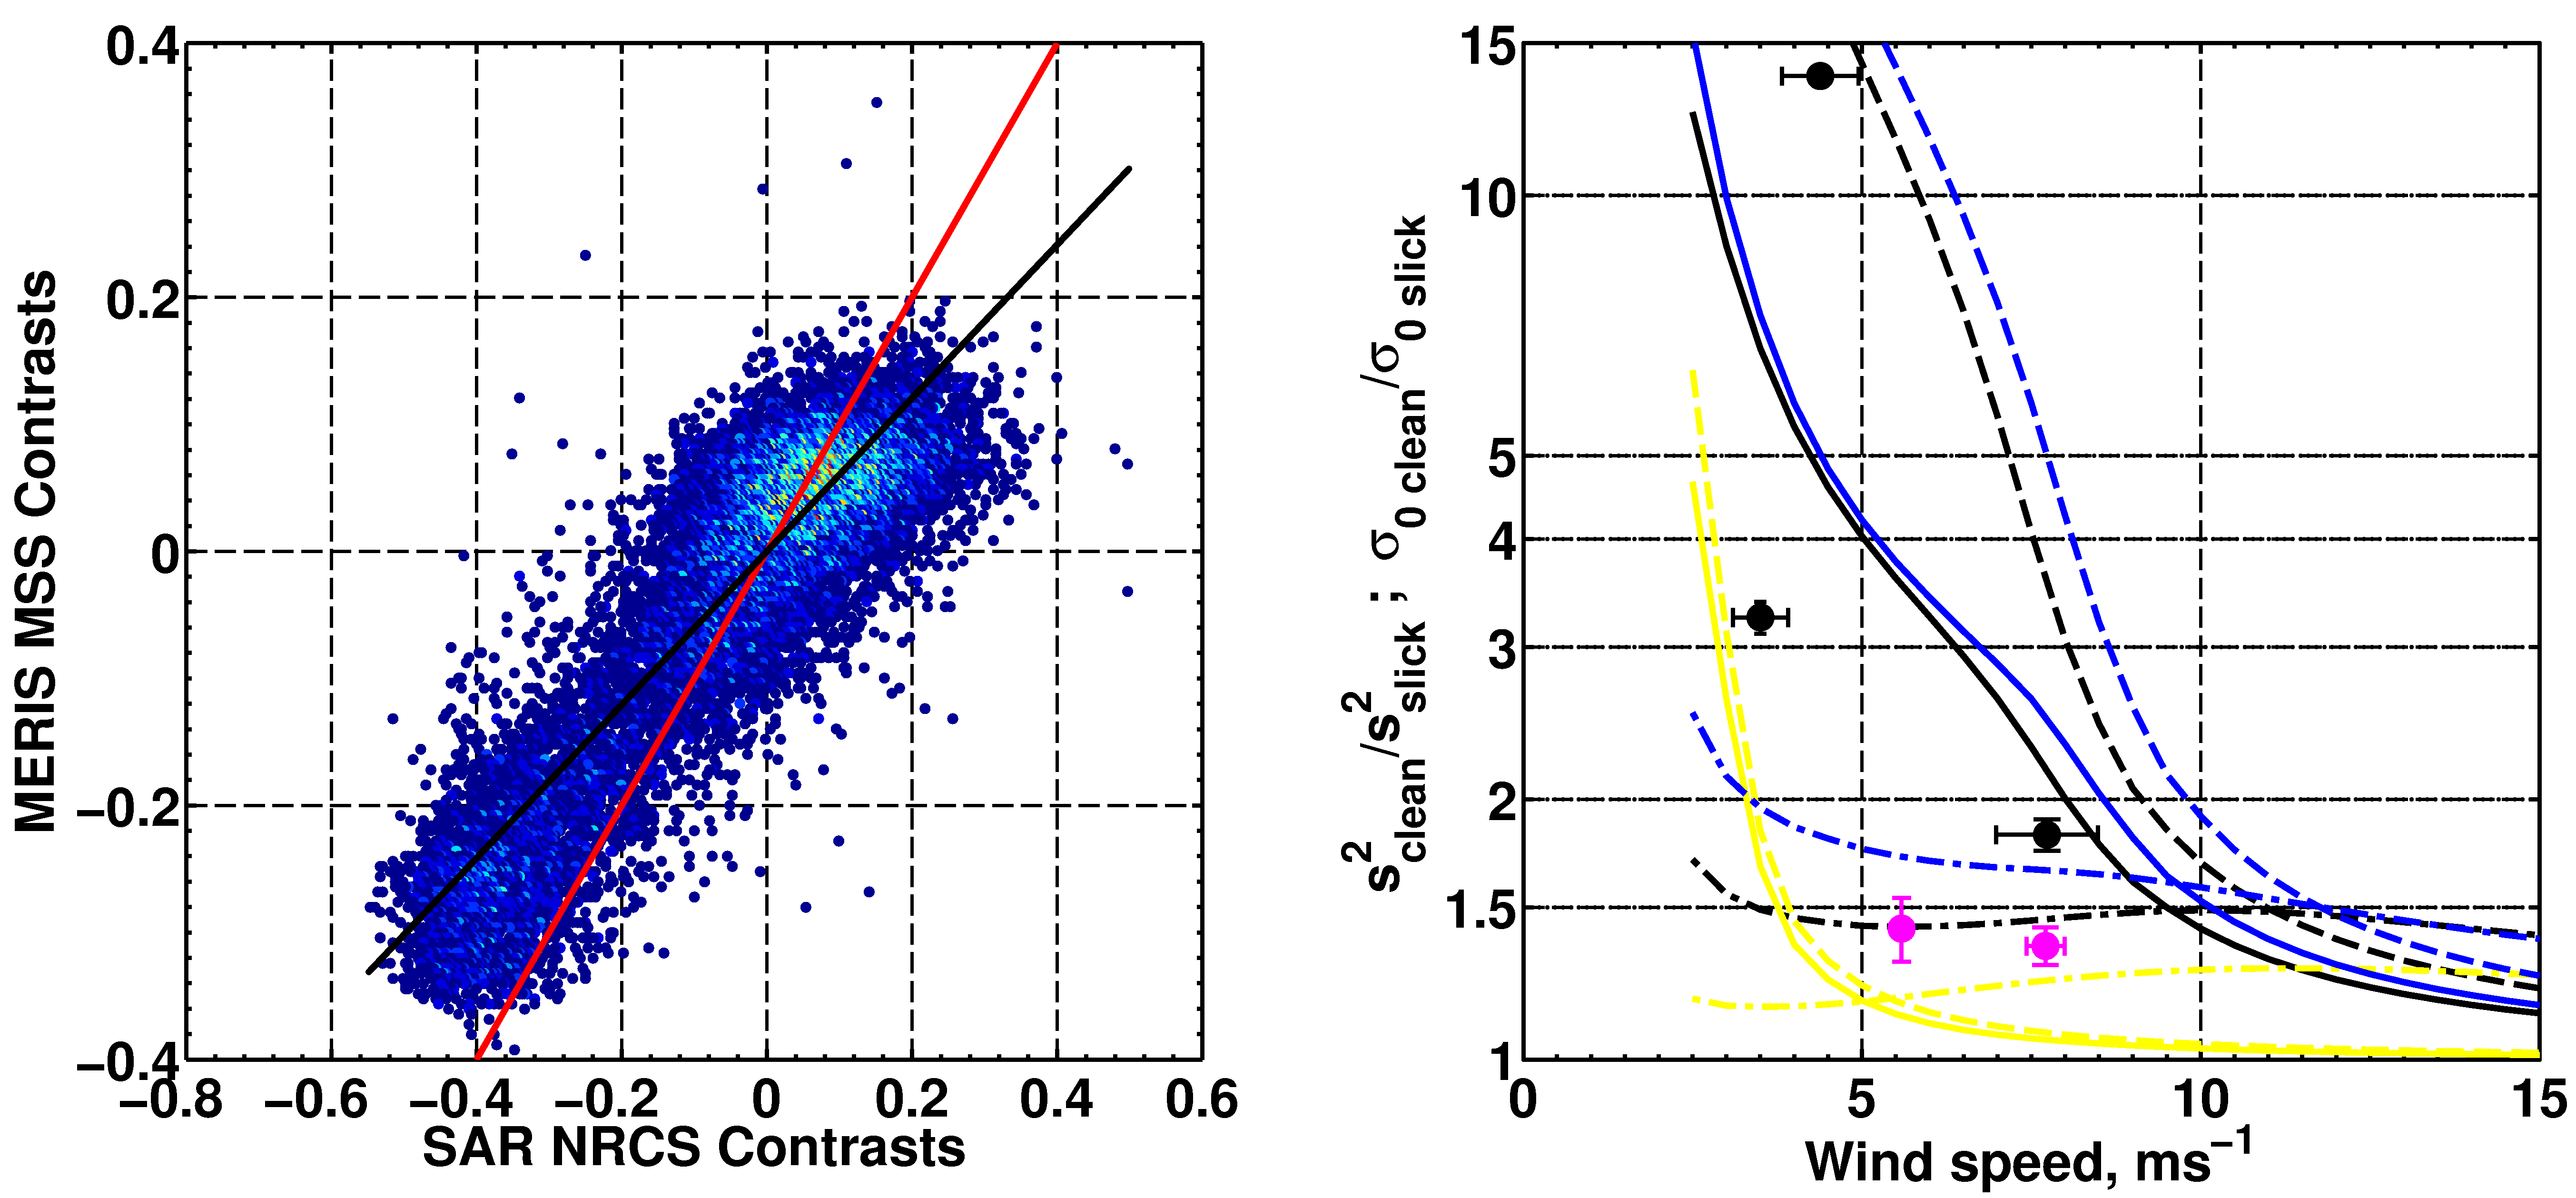
\includegraphics[width=1\linewidth]{fig2_9}}
    \\
    \floattitle{(слева) Отношение контрастов СКН и контрастов УЭПР нефтяного слика в области ``вне'' жёлтого контура, изображённого на Рисунке~\ref{fig:2.8}. Красная линия -- отношение один к одному, а чёрная -- линейная регрессия данных: $\tilde{s}^{2} /s^{2} \approx 0.6\cdot \tilde{\sigma }_{0} /\sigma _{0} $.
    (справа) Чёрная точка с погрешностью в районе значения скорости ветра 7.5\textit{м/с} -- усреднённые контрасты УЭПР нефтяного слика вне жёлтого контура на Рисунке~\ref{fig:2.8b}. Две другие чёрные точки -- контрасты УЭПР того же нефтяного разлива, но полученные по изображению ASAR 25 Мая 2010, 15:47 GMT (здесь не приводятся). Розоватые точки -- усреднённые контрасты СКН, полученные по изображению MERIS на Рисунке~\ref{fig:2.6a}, для нефтяной струи, и на Рисунке~\ref{fig:2.8a} для области вне жёлтого контура. Точка-пунктирные линии -- данные симуляции модели формирования радиолокационных изображений (RIM) контрастов СКН нефтяного слика для E=5, 15, 30\textit{мН/м} (жёлтая, чёрная и синяя линии, соответственно). Результаты RIM симуляций контрастов УЭПР нефтяного слика в рамках ``чисто'' Брэгговской модели рассеяния и полной модели УЭПР, учитывающей эффект обрушений волн на обратное рассеяние радиолокационного сигнала приводятся в виде пунктирных и сплошных линий, соответственно. Пояснения к цветам линий контрастов УЭПР такие же как и у СКН}
    \caption{Контрасты СКН и контрасты УЭПР нефтяного слика вне жёлтого контура, изображённого на Рисунке~\ref{fig:2.8}}
    \label{fig:2.9}
\end{figure}



\section{Контрасты СКН и УЭПР нефтяных сликов} \label{sec:2.3}


В предыдущем разделе предполагается, что представленные на Рисунке~\ref{fig:2.8a} контрасты СКН, заключённые внутри жёлтого контура, соответствуют толстым, в сравнении с длиной волны красного света, нефтяным плёнкам. Показанные же на Рисунке~\ref{fig:2.2} (справа) контрасты СКН, - наоборот, соответствуют тонким. Если предположить, что толщина тонких плёнок, значительно меньше длин капиллярных волн, тогда механизм гашения поверхностных волн тонкими нефтяными плёнками может быть описан в рамках классической теории Марангони \citep{Levich1962}. В этом случае, модуль упругости является единственным параметром, характеризующий свойства подавления тонких нефтяных плёнок и до сих пор остаётся плохо изученным.

Нефтяная плёнка влияет на ветровые волны через изменение коэффициента затухания волн. Соотношение для коэффициента затухания волн в присутствии поверхностных тонких плёнок даётся в \citep{Levich1962}. Вязкая диссипация играет ключевую роль в балансе энергии капиллярно-гравитационных волн. Поэтому, поверхностные плёнки, увеличивая энергию диссипации, должны влиять как на спектр коротких волн, так и на среднеквадратичный наклон (СКН). В данной работе мы используем модель спектра ветровых волн из модели формирования радиолокационных изображений (RIM), предложенной в \citep{Kudryavtsev2003, Kudryavtsev2004, Kudryavtsev2005} и \citep{Johannessen2005}. Основные соотношения модели приводится в  Приложении~\ref{AppendixA}. В модели используется модель спектра волн, который изначально был создан для моделирования спектра волн в фоновых условиях (не подверженных воздействию поверхностных загрязнений), и использовался для анализа данных радиолокационного зондирования морской поверхности. Этот спектр, а так же предложенная в этих работах композитная РЛ модель, учитывающая вклад обрушения волн на РЛ сигнал, была верифицирован на многочисленных экспериментальных данных, и показала вполне удовлетворительное соответствие (см, например, \citep{Mouche2006}). Этот спектр и соответствующая РЛ модель используются в данной работе в исходной форме, без какой-либо специальной модификации или подгонки параметров. Уравнение баланса энергии в равновесном диапазоне гравитационных и капиллярно-гравитационных волн записывается следующим образом:


\begin{equation} \label{eq:2.1}
\beta_{\nu }(k) B(k) - B(k) \left[ B(k) / \alpha \right]^n + I_{wb}(k) = 0 ,
\end{equation}


\noindent где $B({\rm k})$ - спектр насыщения ветровых волн, $\alpha $ и $n$ - модельные параметры, $I_{wb}^{} $ - скорость генерации коротких волн в результате обрушения более длинных волн (включая генерацию паразитных капилляров), $\beta_{\nu } $ - скорость эффективного роста волн



\begin{equation} \label{eq:2.2} 
\beta _{\nu } =c_{\beta } (u_{{\rm *}} /c)^{2} {\rm cos}\varphi |{\rm cos}\varphi |-4\nu k^{2} /\omega ,
\end{equation}


\noindent представляющая разность между ``ветровой накачкой'' энергии (первый член л.ч.) и вязкой диссипацией (второй член л.ч.), $\varphi $ -- угол между векторами скорости ветра и волнового числа, $c$, $\omega $ and ${\rm k}$ фазовая скорость, частота и волновое число, соответственно, $c_{\beta } $ - ``постоянная'' скорости роста ветра (соответствует параметризации Стюарта \citep{Stewart1974}), $u_{{\rm *}} $ - динамическая скорость, $\nu $ - эффективный коэффициент вязкости, учитывающий влияние поверхностной плёнки (для чистой поверхности он соответствует молекулярному коэффициенту вязкости воды $\nu _{0} $). Из уравнения \eqref{eq:2.1} следует, что спектр коротких волн определяется балансом различных источников и стоков энергии, представленных в \eqref{eq:2.1}: притоком ветровой энергии и вязкой диссипацией (первый член), нелинейные потери энергии, включая обрушения волн (второй член), генерацию паразитных капилляров и коротких волн, в результате обрушения более длинных ветровых волн (третий член). Форма волнового спектра следует из решения уравнения \eqref{eq:2.1} (подробнее см. \citep{Kudryavtsev2005}).

Влияние поверхностных плёнок на спектр волн проявляется через модификацию коэффициента вязкости в первом члене уравнения баланса энергии \eqref{eq:2.1}.
Коэффициент эффективной вязкости поверхности воды, покрытой тонкой поверхностной плёнкой с упругостью $E=$5, 15, и 30\textit{мН/м,} нормированной на коэффициент вязкости воды представлен на Рисунке~\ref{fig:2.10},~а. С увеличением упругости плёнки, величина коэффициента эффективной вязкости увеличивается и его пик смещается в сторону более длинных волн. Увеличение вязкой диссипации нарушает баланс энергии \eqref{eq:2.1} и приводит к подавлению спектральной энергии в высокочастотной части спектра. Спектры коротких волн, проинтегрированные по всем направлениям на чистой поверхности и в присутствии поверхностных плёнок, показаны на Рисунке~\ref{fig:2.10},~б. Особенностью спектров волн в присутствии плёнок является резкое падение энергии в высокочастотной области спектра, которая смещается в область низких частот с увеличением упругости. Эта спектральная ``отсечка'' связана с пересечением нуля эффективным ростом волн \eqref{eq:2.2}, когда вязкая диссипация (зависящая от $E$) превышает приток ветровой энергии. Волновое число спектральной отсечки $k_{cut} $ может быть рассчитан из решения уравнения $\beta _{v} (k_{cut} )=0$. СКН морской поверхности определяется через спектр насыщения как



\begin{equation} \label{eq:2.3} 
s^{2} =\mathop{\smallint }\limits_{k}^{} B\left(k\right)d{\rm ln}k 
\end{equation} 


Как следует из этого уравнения, СКН должен быть чувствителен к волновому числу спектральной отсечки, а следовательно, - и к упругости нефтяной плёнки. В этом случае СКН в слике могут являтся источником информации о его природе. Также стоит обратить внимание на локальный высокочастотные спектральные пики в спектре насыщения для плёнок с упругостями \textit{E}=5 и 15\textit{мН/м}. Эти пики являются следствием генерации паразитных капилляров в результате обрушения коротких гравитационных волн. Для \textit{E}=30\textit{мН/м}, эти короткие гравитационные волны значительно подавляются плёнкой, которая предотвращает генерацию паразитных капилляров.



\begin{figure}[!ht]
   	\centering
	{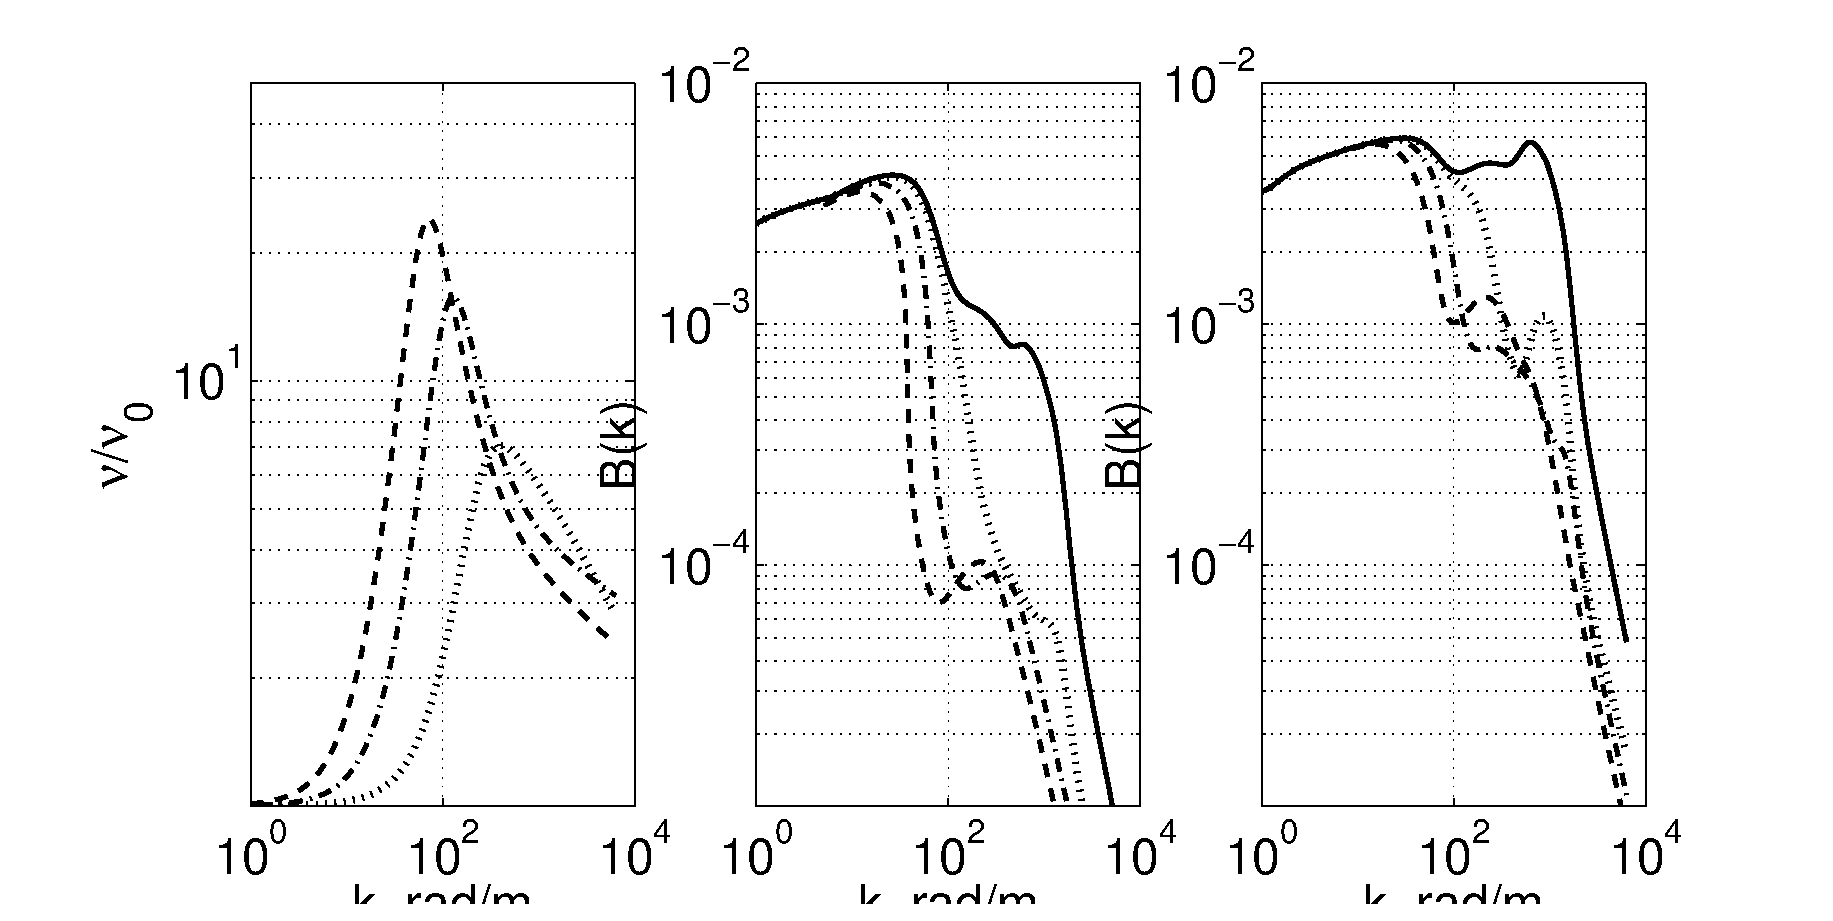
\includegraphics[width=\linewidth]{fig2_10}}
    \\
    \floattitle{(а) Коэффициент гашения волн, $\nu $, масштабированный на вязкость воды, $\nu _{0} $, для плёнок различной эластичности, $E$,: E=5\textit{мН/м} (штрих-пунктир), E=15\textit{мН/м} (пунктир), и E=30\textit{мН/м} (сплошная). (б) Спектр насыщения ветровых волн для чистой поверхности (жирная сплошная, исходный спектр), и для поверхности, покрытой плёнкой с упругостью E=5\textit{мН/м} (штрих-пунктир), E=15\textit{мН/м} (пунктир), и E=30\textit{мН/м} (тонкая сплошная)}
    \caption{Коэффициент затухания волн и спектр насыщения ветровых волн для различных условий}
    \label{fig:2.10}
\end{figure}


Упругость тонкой плёнки нефтепродуктов мало изучена, поэтому, для оценки свойств нефтяной плёнки по наблюдаемым контрастам СКН, мы предлагаем использовать спектральную модель \eqref{eq:2.1}, совместно с определённым по \eqref{eq:2.3} СКН. Жёлтая, чёрная и синяя кривые на Рисунке~\ref{fig:2.2}~(справа) показывают результаты моделирования контрастов СКН для плёнок с упругостями $E=$5, 15, и 30\textit{мН/м.} Несмотря на то, что разброс данных достаточно большой, модельные расчёты для $E=15$\textit{мН/м} дают наилучшее соответствие с данными. Это значение упругости существенно отличается от $E=4$\textit{мН/м,} использованное в статьях по изучению нефтяных сликов (см., например, \citep{2008}).

На Рисунке~\ref{fig:2.9} (справа) представлены результаты модельных расчётов контрастов УЭПР (С-диапазон, ВВ поляризация, направление визирования против ветра, угол падения 30${}^\circ$) для поверхности, покрытой нефтяными плёнками, с упругостями $E=$5, 15, и 30\textit{мН/м.} Контрасты УЭПР рассчитывались для двух моделей рассеяния: ``чисто'' Брэгговское рассеяние ${\sigma}_{0{br}}^{pp}$, и композитная модель, учитывающая радиолокационное рассеяние от обрушающихся волн ${\rm \sigma }_{0}^{pp} ={\rm \sigma }_{0{\rm br}}^{pp} +{\rm \sigma }_{0{\rm b}} $, где $\sigma _{0b} $ представляет вклад обрушений волн в обратное рассеяние РЛ-сигнала. Для первой модели, контрасты УЭПР соответствуют контрастам волнового спектра на Брэгговском волновом числе $k_{br} $ (см. спектр на Рисунке~\ref{fig:2.10},~б, $k_{br} =10^{2}$ \textit{рад/м}). Для другой же модели, контрасты УЭПР сочетают подавление Брэгговского волнового спектра и обрушений волн. Следуя модели, диапазон обрушающихся волн, обеспечивающих не-брэгговское рассеяние, определяется как $k<k_{R} /10$. Для радиолокатора C-диапазона, это соответствует длинам волн $>$ 60\textit{см}. Как следует из Рисунка~\ref{fig:2.10},~б, эти волны не подвержены влиянию гашения нефтяной плёнкой, и контрасты УЭПР, предсказанные моделью, ниже, чем в случае ``чисто'' Брэгговской модели рассеяния. Если волновой спектр при $k=k_{br} $ значительно подавляется в области слика (как это видно из Рисунков~\ref{fig:2.10},~б и \ref{fig:2.9} (справа) для плёнок с $E=$ 15 и 30\textit{мН/м }), Брэгговский механизм рассеяния ``отключается'' и УЭПР формируется в основном за счёт обрушений. В таком случае, отношение УЭПР для чистой и сликовой поверхностей, ${\rm \sigma }_{0{\rm clean}}^{pp} /{\rm \sigma }_{0{\rm slick}}^{pp} $, в основном соответствует обратному отношению вкладу обрушений волн в полную УЭПР чистой поверхности, т.е. ${\rm \sigma }_{0{\rm clean}}^{pp} /{\rm \sigma }_{0{\rm slick}}^{pp} \approx {\rm \sigma }_{0}^{pp} /{\rm \sigma }_{0{\rm b}} $.

Осреднённые контрасты УЭПР для нефтяных сликов показанных ранее на Рисунке~\ref{fig:2.8b}, представлены на Рисунке~\ref{fig:2.9} (справа) вместе со средними контрастами УЭПР, полученным по данным ASAR. Экспериментальные оценки хорошо соответствуют модельным расчётам как для $E$=15\textit{мН/м}, так и для $E$=30\textit{мН/м}. Одинаковые значения контрастов УЭПР при существенных разностях упругостей получаются потому, что коэффициент гашения волн при $k_{br} =10^{2}$\textit{рад/м} для этих значений упругости оказывается одинаков (см. Рисунок~\ref{fig:2.10},~а). В этом случае не удаётся разделить поверхностные слики с различной упругостью по контрастам УЭПР.

Как показано в работе \citep{2008}, в результате сложной формы спектральных контрастов, приведённых на Рисунке~\ref{fig:2.10}, контрасты УЭПР сильно зависят от ``геометрии'' РЛ-наблюдений (длины волны, угла наблюдения, направления визирования), что делает практически трудно разрешимой задачу разделения и интерпретации плёнок различного происхождения (биогенные плёнки, нефтяные и др. слики).

Напротив, контрасты СКН зависят от спектральной отсечки, которая напрямую связана с упругостью поверхностной плёнки, в свою очередь, зависящей от её происхождения. С этой точки зрения, данные оптических наблюдений поверхностных сликов могут дать нам возможность разделить плёнки биогенного происхождения (ожидаемая упругость 25-30\textit{мН/м }) и слики нефтепродуктов, которые (следуя нашим оценкам) имеют упругость около \textit{15мН/м}.



\newpage



\section{Выводы по главе}


Предложенный в Главе~\ref{chap:1} метод восстановления контрастов среднеквадратичного наклона (СКН) применён к анализу проявления нефтяных сликов естественного и техногенного происхождения, на изображениях солнечного блика, полученных приборами MODIS и MERIS.

Показано, что контрасты яркости сликов могут быть как положительными, так и отрицательными. Это свойство следует непосредственно из геометрии наблюдения, когда формируется так называемая зона инверсии контрастов. Хотя это свойство является естественным ``строгим'' следствием модели формирования контрастов СКН в блике, этот факт в зарубежной литературе отмечается как неожиданный.

В результате анализа спутниковых изображений показано, что разработанные алгоритмы дают возможность оценить пространственное распределение поверхностных загрязнений, и оценить контрасты СКН в сликах, которые определяются физико-химическими свойствами поверхностных пленок.

Установлено, что контрасты СКН в нефтяных сликах несколько ниже контрастов СКН в сликах биологического происхождения. Этот результат можно объяснить различной упругостью нефтяных плёнок и плёнок биологического происхождения.

Было обнаружено, что в тех районах нефтяных загрязнений, где толщина нефтяной плёнки значительно превышает длину волны красного света, восстановленные значения аномалий СКН противоречат ожидаемому эффекту подавления коротковолнового волнения в сликах. Сделан вывод, что в этом случае контрасты яркости морской поверхности определяются ``цветом'' нефти, что не учитывалось в методе.

Для интерпретации наблюдаемых контрастов СКН в сликах использовалась модель спектров коротких волн, предложенная в работах \citep{Kudryavtsev2005, 2008}. Получено, что модельные контрасты согласуются с наблюдениями в том случае, если эффективный коэффициент упругости равен $E$=15\textit{мН/м}.

Синхронные ASAR РСА и оптические изображения дали возможность проанализировать подобие и различия между проявлениями одних и тех же нефтяных сликов. Показано, что оптические и РЛ-контрасты одного и того же слика, сформированного тонкой нефтяной плёнкой, хорошо коррелируют. При этом радиолокационные контрасты примерно в 1.6 раза сильнее контрастов СКН. Моделирование контрастов УЭПР по модели, описанной в \citep{2008}, показали, что значение упругости $E$=15\textit{мН/м} для нефтяной плёнки также обеспечивает хорошее соответствие модельных оценок и измерений.

Показано, что при совместном анализе контрастов яркости морской поверхности в солнечном блике и РСА контрастов в сликах, можно сделать качественное заключение о толщине пленки.



\clearpage